\chapter{Technologien und Werkzeuge}
\label{chap:technologies}

%%%%%%%%%%%%%%%%%%%%%%%%%%%%%%%%%%%%%%%%%%%%%%%%%%%%%%%%%%%%
\section{Bluetooth 4.0}
\label{sec:technologies:bluetooth4}
%%%%%%%%%%%%%%%%%%%%%%%%%%%%%%%%%%%%%%%%%%%%%%%%%%%%%%%%%%%%

Der Bluetooth-Standard 4.0, auch Bluetooth Smart genannt, wurde am 30.Juni 2010 verabschiedet. Darin enthalten sind alle Protokolle der vorherigen Version 3.0, sowie Fehlerkorrekturen und Erweiterungen \cite{bluetoothcore}. Außerdem wurde ein neues Protokoll hinzugefügt, Bluetooth Low Energy. 

Das erste unterstützte Mobilfunkgerät war das iPhone 4s \cite{iphone4sspecs}, welches am 4. Oktober 2011 vorgestellt wurde. Im Jahr 2012 integrierten auch andere Smartphone-Hersteller Bluetooth 4.0 in ihre Geräte, sodass alle neueren Geräte diesen Standard beherschen.


%%%%%%%%%%%%%%%%%%%%%%%%%%%%%%%%%%%%%%%%%%%%%%%%%%%%%%%%%%%%
\subsection{Bluetooth Low Energy}
\label{sec:technologies:bluetoothLE}
%%%%%%%%%%%%%%%%%%%%%%%%%%%%%%%%%%%%%%%%%%%%%%%%%%%%%%%%%%%%

Bluetooth Low Energy wurde Anfangs von Nokia unter dem Namen ''Wibree'' entwickelt. Die Zielsetzung dabei war es eine Technologie zu entwickeln, mit der sich Computer und Mobilgeräte schnell und einfach mit Peripherie-Geräten verbinden lassen sollten. Das Hauptaugenmerk galt dabei dem geringen Stromverbrauch, einer kompakten Bauweise und den geringen Kosten der benötigten Hardware.
Im Jahr 2007 wurden diese Spezifikationen in den, sich in der Entwicklung befindlichen, Bluetooth-Standard 4.0 aufgenommen. Wibree wurde daraufhin in Bluetooth Low Energy, oder kurz BLE, umbenannt \cite{wibree}.

Bluetooth Low Energy arbeitet wie das klassische Bluetooth im 2,4 GHz Band, bringt aber in der Funktionsweise einige Unterschiede mit sich.

So wurde, im Vergleich zum klassischem Bluetooth, die Datenrate von bis zu 3 Mbit/s auf maximal 1 Mbit/s reduziert. Dies führt dazu, dass BLE beispielsweise nicht für Headsets genutzt werden kann, da die zur Verfügung stehende Übertragungsrate nicht für eine Audioübertragung ausreicht.

Die Vorteile die BLE dabei mit sich bringt, liegen vor allem in der niedrigen Latenz, welche von 100ms auf weniger als 3ms reduziert wurde, und dem drastisch gesenkten Energieverbrauch im Vergleich zu den Vorgänger-Versionen. Der gesenkt Energieverbrauch hängt dabei mit verschiedenen Faktoren zusammen. 
Dabei wurde unteranderem die maximale Paketgröße auf 20 Byte verringert. Außerdem wurden die Empfangs- und Sendefenster verkleinert. 
Darüberhinaus arbeitet BLE nach dem Race-to-idle Prinzip. Dabei werden anstehende Daten schnellstmöglich gesendet und das Gerät geht, sobald die Daten verschickt worden sind, direkt in den Schlafmodus bis neue Daten vorliegen.

Eine weitere Neuerung ist die Nutzung einer 24-Bit-Fehlerkorrektur, welche die Verbindung unempfindlicher gegenüber Störungen und Übertragungsfehlern machen soll und so unnötige Neuübertragungen verhindert.

Auch die Verschlüsselung des zu übertragenden Signals wurde verbessert. Dabei kommt der Advance Encryption Standard (AES) mit einer Schlüssellänge von 128 Bit zum Einsatz (vgl. \cite{blespecs}. 

Das Bluetooth Low Energy Architektur besteht dabei aus verschiedenen Schichten und Komponenten \cite{blespecsnordic}.

\textbf{Central und Peripheral}
Bei einer Bluetooth Low Energy-Verbindung unterscheidet man zwischen \emph{Central} und \emph{Peripheral}. Das Gerät in der Rolle des \emph{Central} horcht dabei auf gesendete Pakete von verbundenen oder allen in der Umgebung befindlichen Geräten. Das Gerät in der Rolle des \emph{Peripheral} hingegen sendet Pakete an die verbundenen oder an alle Geräte.


\textbf{ATT}
Das \emph{Attribute Protocol}, oder kurz \emph{ATT}, wird bei allen Datenübertragungen mittels Bluetooth Low Energy genutzt. Es wurde speziell für Bluetooth LE entworfen, um eine schnelle und sparsame Übertragung zu ermöglichen. 
Ein Attribut-Paket des ATT besteht dabei aus drei Bestandteilen. Einem 16 Bit \emph{Handle}, einem 128 Bit \emph{Universally Unique Identifier (UUID)} und einem \emph{Value} mit variabler Länge.
Der \emph{Handle} ist eine Nummer, welche das Attribut eindeutig identifiziert, da mehrere Attribute mit gleichem UUID möglich sind.
Der \emph{UUID} beschreibt den Typ des gesendeten Attributes, wobei die verschiedenen UUID's nicht im ATT festgelegt werden, sondern in darüberliegenden Profilen wie etwa GATT.
Die Länge des \emph{Value's} hängt dabei von dem Typ des gesendeten Attributes ab, lässt sich also in höheren Protokollen aus dem UUID bestimmen.

Das ATT basiert dabei auf einer Client-Server-Architektur, wobei nur der Server Attribute speichert und der Client diese ausliest oder schreibt.

\textbf{GATT}
Das \emph{Generic Attribute Profile (GATT)} ist verpflichtend für alle Bluetooth LE-Profile. Es basiert dabei auf ATT und erlaubt ein einfache und geregelte Übertragung der Attribute. Ein Beispiel für ein GATT-Profil ist das \emph{Heart Rate Profile}, welches für Herzfrequenzmessungen designt wurde.
Jedes Profil besteht dabei aus verschiedenen Attributen, welche hierarchisch aufgebaut sind.
Die einzelnen Attribut-Typen unterscheiden sich dabei durch ihre UUID, welche in den GATT-Profilen eindeutig festgelegt sind.

An oberster Stelle steht dabei das \emph{Service}-Attribut. Ein Service besteht aus einer Menge von \emph{Characteristics}. Eine Beispiel für einen GATT-Service ist der \emph{Heart Rate Service}, welcher aus mehreren \emph{Characteristics} besteht, wie zum Beispiel der \emph{Heart Rate Measurement Characteristic}, welche die aktuelle Herzfrequenz beschreibt oder der \emph{Body Sensor Location Characteristic}, welche die Lage des Herzfrequenzmessers beschreibt. 
Das \emph{Characteristic}-Attribut besteht aus einem Messwert und einem \emph{Descriptor}. Der aktuelle Wert ist abhängig von der Characteristic, so gibt die \emph{Heart Rate Measurement Characteristic} beispielsweise die aktuelle Herzfrequenz als Wert zurück. 
Der \emph{Descriptor} liefert zusätzliche Information über die aktuelle \emph{Characteristic}, wie zum Beispiel den erlaubten Wertebereich oder die Einheit in welcher der Messwert vorliegt.

\begin{figure}[htb!]
		\centering
	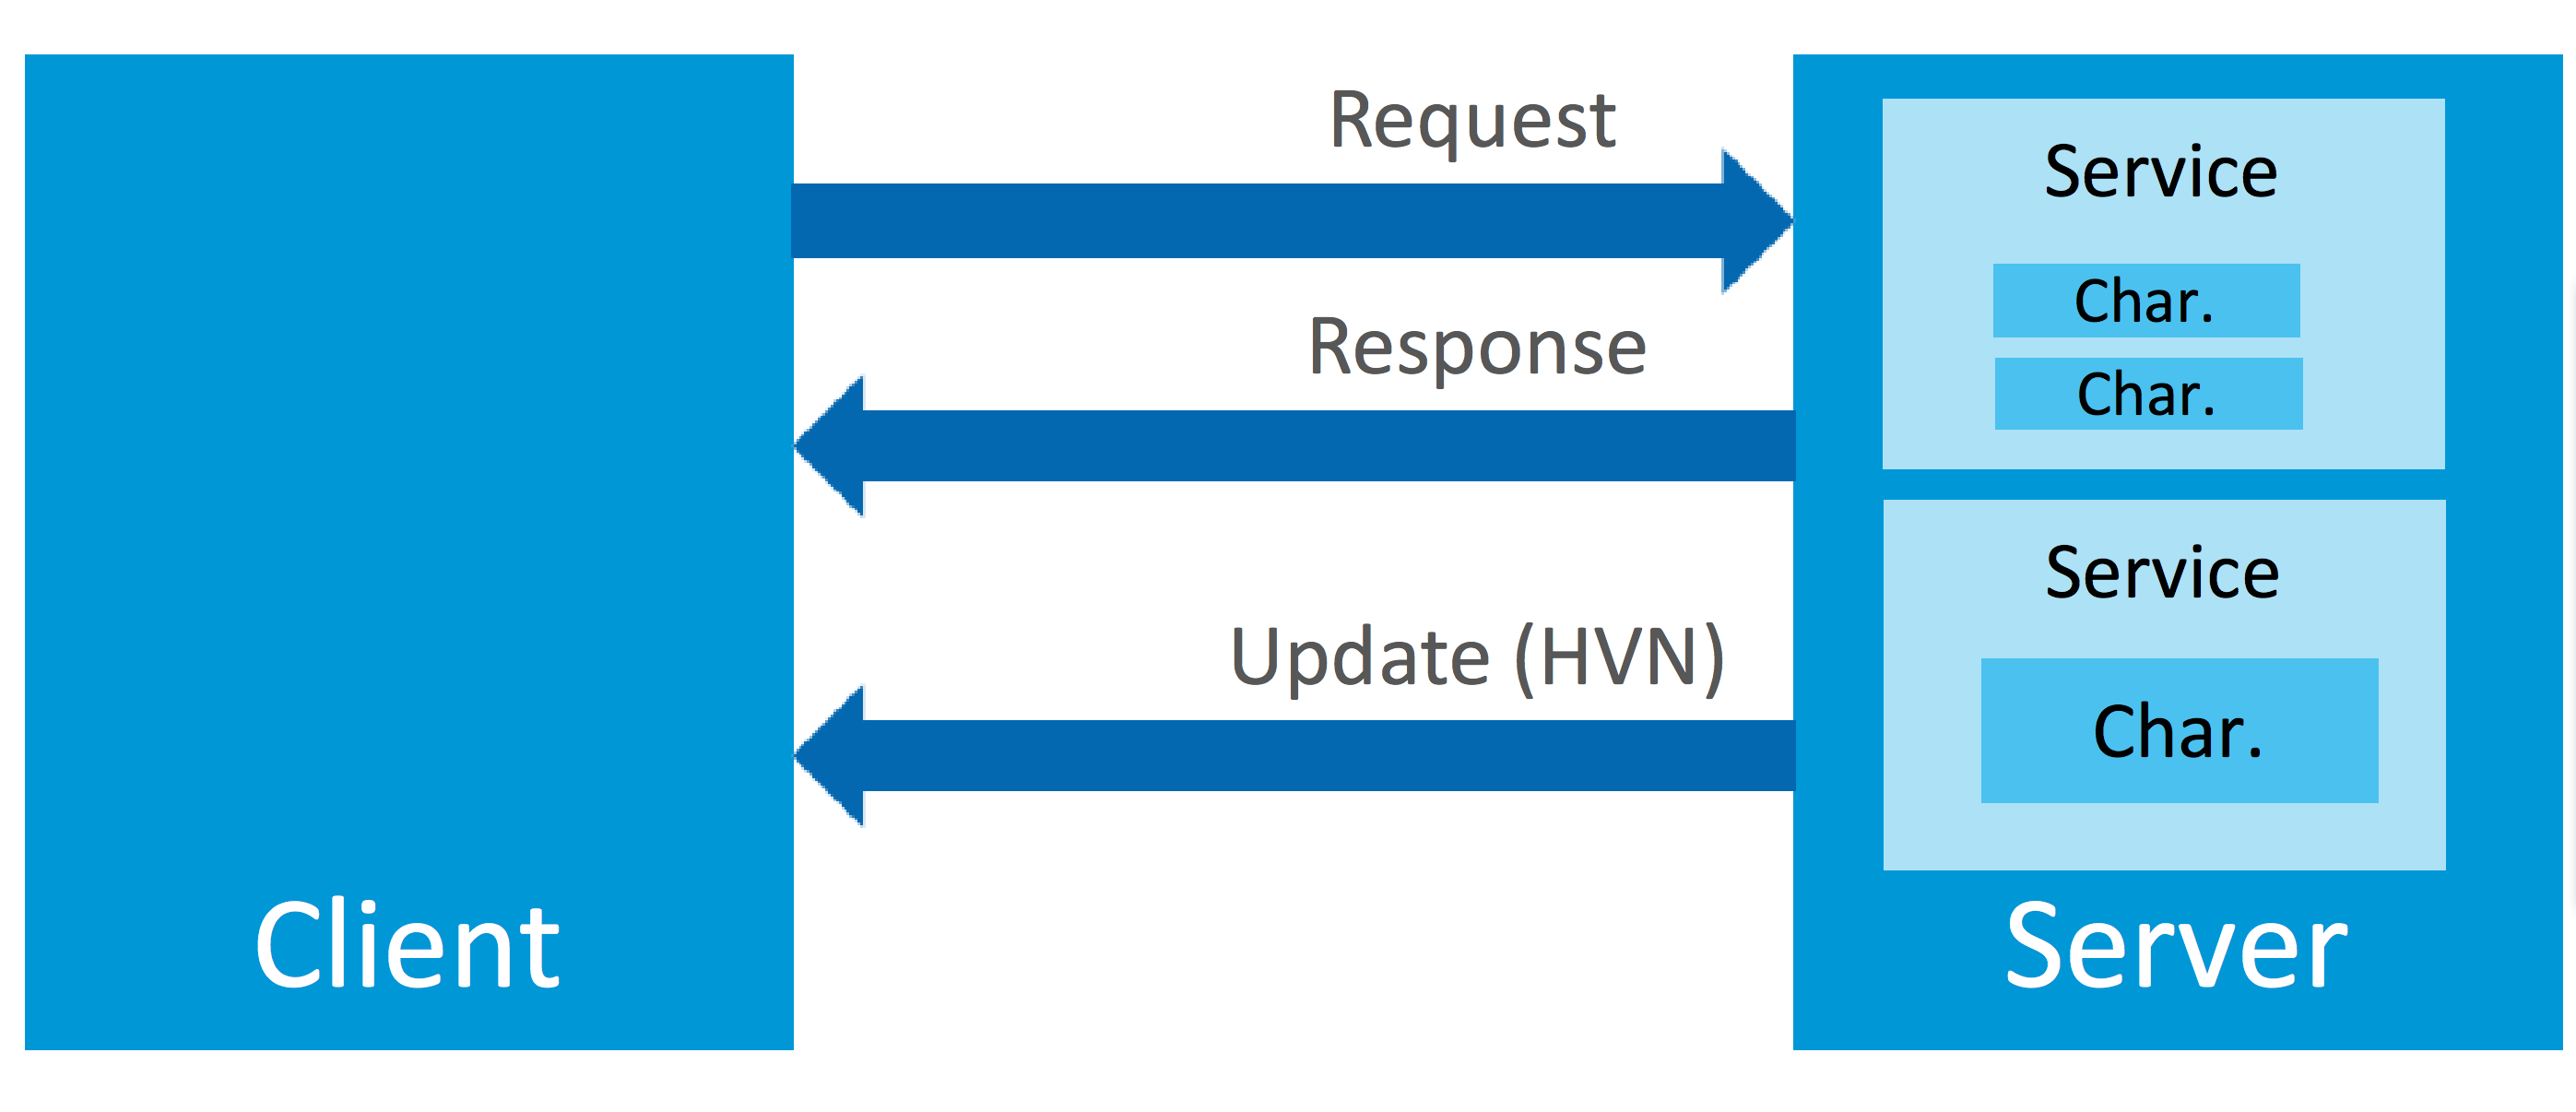
\includegraphics[scale=0.3]{nordic-gatt-overview}
	\caption{Verbindung zwischen Client und Server bei GATT-Übertragung}
	\label{nordic-gatt-overview}
	\end{figure}


%%%%%%%%%%%%%%%%%%%%%%%%%%%%%%%%%%%%%%%%%%%%%%%%%%%%%%%%%%%%
\subsection{iBeacons}
\label{sec:technologies:bluetoothLE:ibeacons}
%%%%%%%%%%%%%%%%%%%%%%%%%%%%%%%%%%%%%%%%%%%%%%%%%%%%%%%%%%%%
Die iBeacons-Technologie wurde am 10.Juni 2014 von Apple auf der Worldwide Developers Conference vorgestellt \cite{appleinsideribeacons}. 
Diese basiert auf Bluetooth Low Energy und arbeitet mit einem von Apple entwickelten, proprietären GATT-Profil.

Beacon bedeutet übersetzt ''Leuchtfeuer'' und die Funktionsweise der Beacons ist dem sehr ähnlich.
Einmal in Betrieb genommen, sendet das Beacon dauerhaft, in kleinen Zeitintervallen, ein Signal in welchem sich Daten zur Identifizierung und Entfernungsbestimmung des Beacons befinden.

Für die Identifizierung sendet das Beacon drei Werte, den \emph{Universally Unique Identifier (UUID)}, den \emph{Major}-Wert und den \emph{Minor}-Wert.
Der \emph{UUID} ist ein Identifier, welcher Beacons einem bestimmten Typ oder einem Unternehmen zuordnen. Dieser UUID lässt sich mittels diversen Programmen generieren \cite{uuidgen}.

Der \emph{Major}-Wert dient zur Unterscheidung von Beacons mit dem selben UUID und wird dazu eingesetzt, verschiedene Standorte beziehungsweise Regionen zu unterscheiden. Ein Beispiel dafür wäre ein Unternehmen mit mehreren Standorten, sodass bei gleichem UUID eine eindeutige Bestimmung des Standortes möglich ist.

Der \emph{Minor}-Wert dient zur weiteren Unterscheidung der Beacons mit gleichem UUID und Major-Wert. Vorgesehen ist der Minor-Wert zur Bestimmung eines einzelnen Beacons in einer bestimmten Region, es ist jedoch nicht verboten mehreren Beacons die gleichen UUID, Major und Minor-Werte zu zuweisen, wodurch jedoch keine eindeutige Identifizierung mehr möglich ist. 

Neben den von Beacon gesendeten Identifikationsdaten kann das Empfangsgerät selbst noch weitere Größen bestimmen. Es ist so zum Beispiel möglich die ungefähre Entfernung zu erhalten. 
Dafür wir der \emph{Proximity}-Wert genutzt. Dieser definiert vier verschiedene Entfernungs-Zustände : \textit{Far(mehr als 10m)}, \textit{Near(wenige Meter)}, \textit{Immediate (wenige Zenitmeter)} und \textit{Unknown(Entfernung konnte nicht bestimmt werden)}. 
Diese Werte erlauben eine sehr grobe Entfernungseinschätzung zum Beacon. 
Für eine differenziertere Entfernungsbestimmung lässt sich eine weitere Kennzahl bestimmen, der \textit{Accuracy}-Wert. Dabei handelt es sich um eine ungefähre Entfernungsangabe in Metern, welche jedoch ausdrücklich nur zur Differenzierung der Enterfernung zweier Beacons genutzt werden soll und keinesfalls einen genauen Abstand zum Beacon angibt. Der Accuracy-Wert soll dabei erlauben, bei gleichem Proximity-Wert, das nächstgelegene Beacon zu bestimmen \cite{clbeaconref}.

\begin{figure}[htb!]
		\centering
	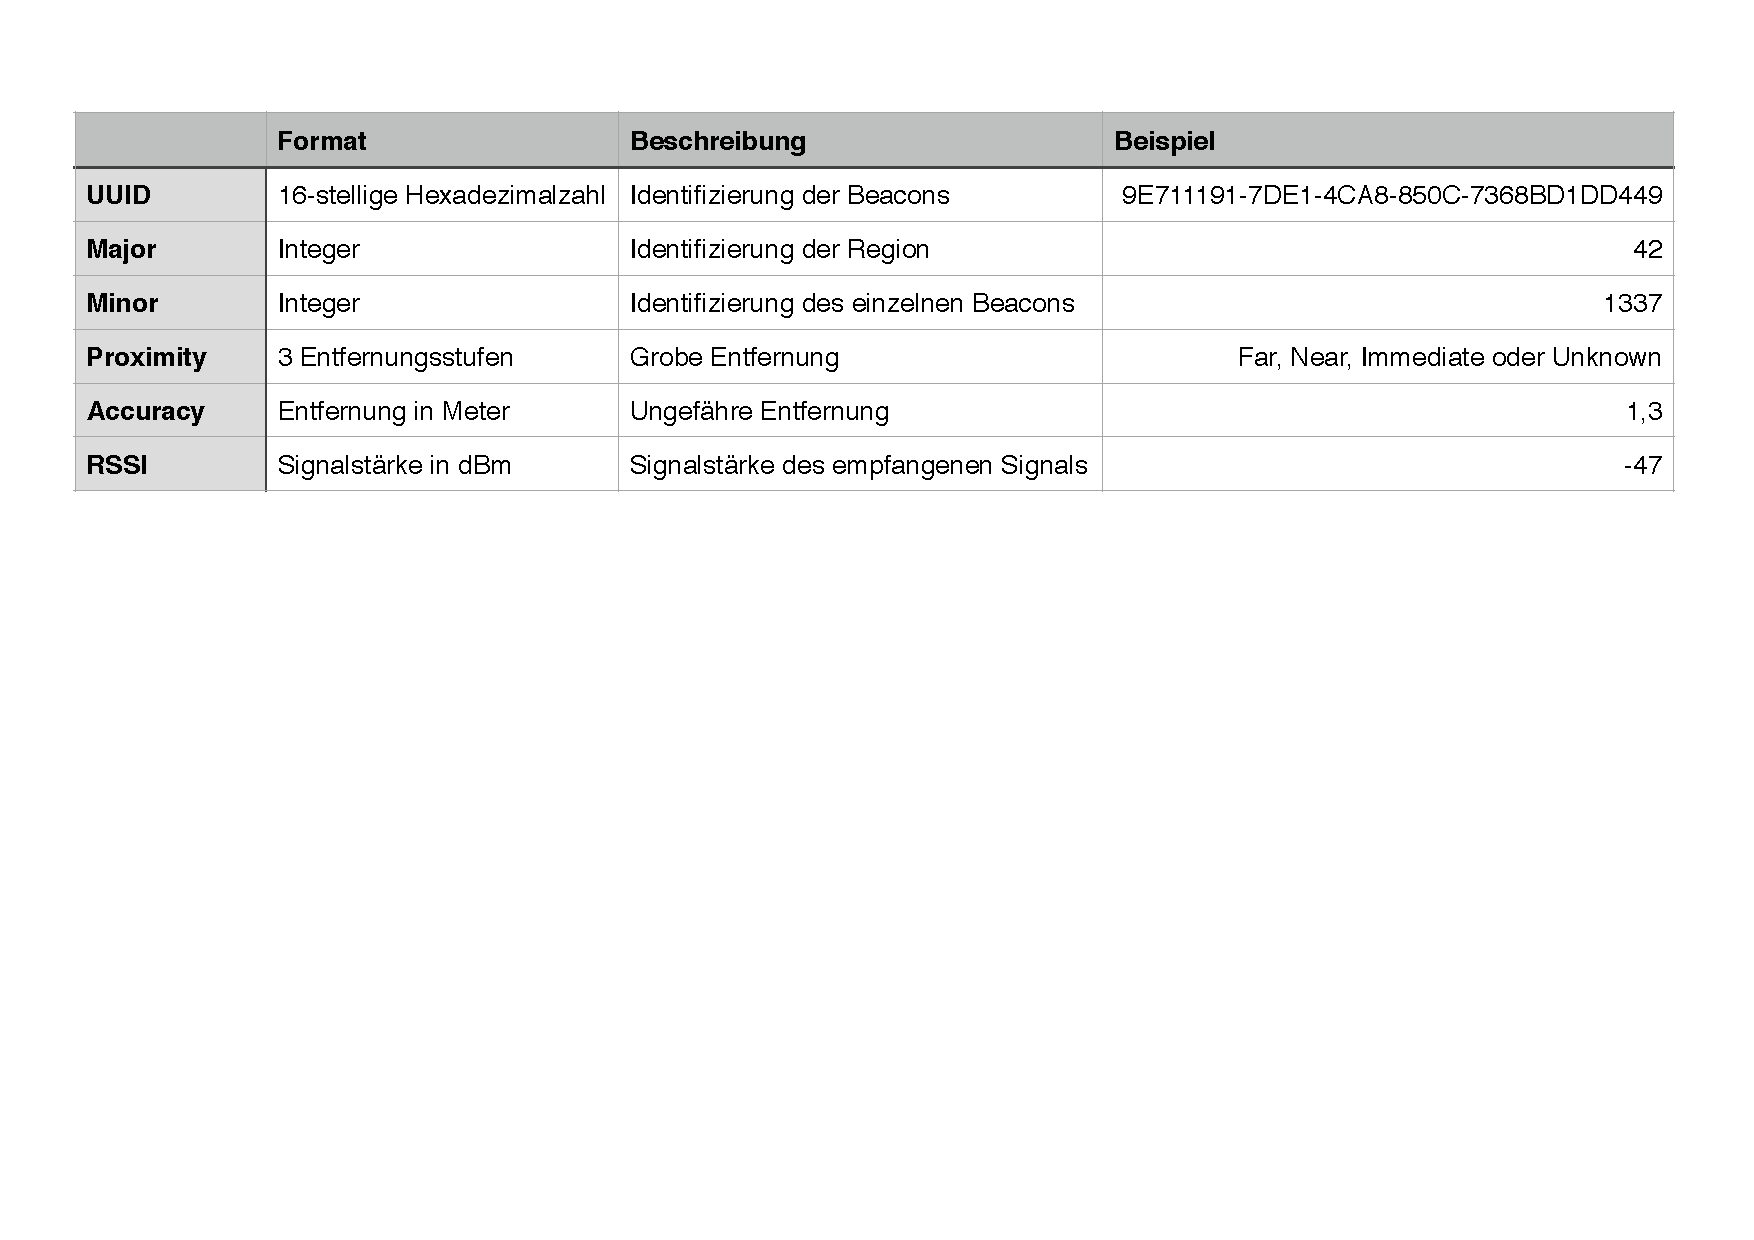
\includegraphics[scale=0.5]{ibeacon-table}
	\caption{Beacon-Daten beim Empfangsgerät}
	\label{ibeacon-table}
\end{figure}


Die von dem Beacon gesendeten Daten lassen sich mit jedem BLE-kompatiblem Gerät empfangen, bisher bietet jedoch nur iOS eine entsprechende, native Unterstützung für das iBeacon-Profil.

Die großen Vorteile der iBeacons sind ihr kleiner Formfaktor, welcher es erlaubt die Beacons an fast jedem beliebigem Ort anzubringen, und ihr geringer Stromverbrauch, der es möglich macht, die Beacons mit einer Knopfzellen-Batterie zu betreiben und das, laut Herstellerangaben, für bis zu zwei Jahre.
Der Aufbau eines solchen Beacons lässt sich in Abbildung \ref{estimote-beacon} erkennen. Den Großteil des Beacons nimmt dabei die Batterie ein. 


%%%%%%%%%%%%%%%%%%%%%%%%%%%%%%%%%%%%%%%%%%%%%%%%%%%%%%%%%%%%
% figure of estimote beacon
%%%%%%%%%%%%%%%%%%%%%%%%%%%%%%%%%%%%%%%%%%%%%%%%%%%%%%%%%%%%
\begin{figure}[h!]
	\centering
	\begin{minipage}[t]{5cm}
		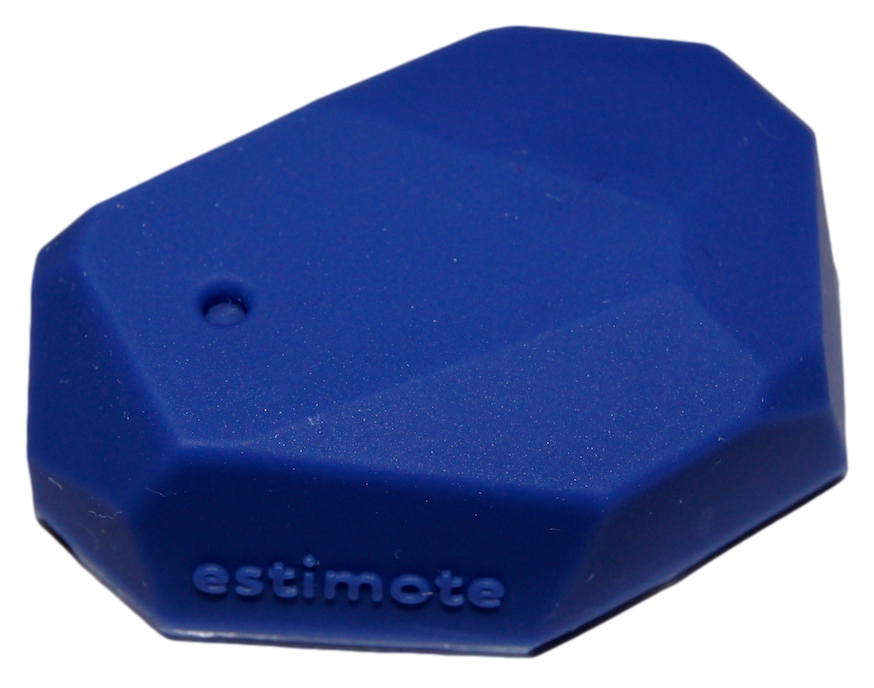
\includegraphics[scale=0.15]{pictures/estimote-beacon-outside}
		\caption{Außenhülle}
		\label{estimote-outside}
	\end{minipage}
	\hspace{2cm}
	\begin{minipage}[t]{5cm}
			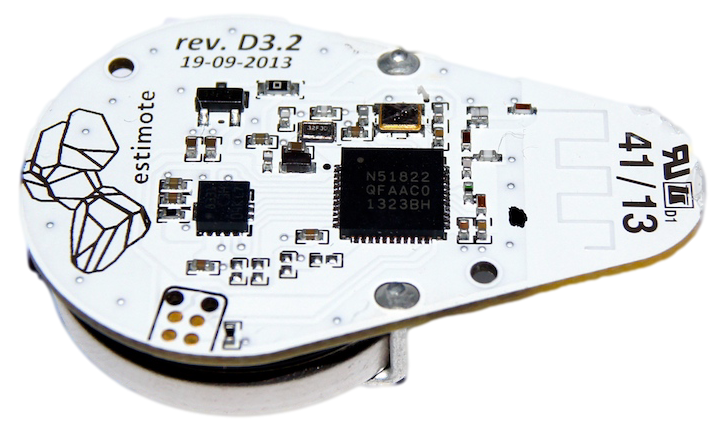
\includegraphics[scale=0.2]{pictures/estimote-beacon-inside}
			\caption{Chipsatz mit Bluetooth-Modul}
			\label{estimote-inside}
	\end{minipage}
		\caption{Ein iBeacon der Firma ''estimote''}
		\label{estimote-beacon}
\end{figure}


Unter genauerer Betrachtung der Platine in Abbildung \ref{estimote-beacon-inside-annotations}, erkennt man, dass diese im Grunde aus zwei Teilen besteht.
Dem Bluetooth-Chipsatz, welcher an sich ist nur wenige Zentimeter groß ist und der Antenne, welche im vorderen Bereich der Platine eingearbeitet ist und über die letztendlich die Daten gesendet werden.

\begin{figure}[h!]
	\centering
	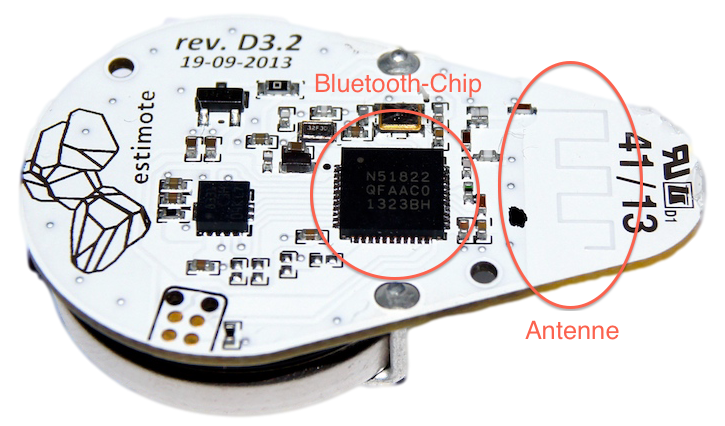
\includegraphics[scale=0.25]{estimote-beacon-inside-annotation}
	\caption{Aufbau des estimote-Beacons}
	\label{estimote-beacon-inside-annotations}
\end{figure}



%%%%%%%%%%%%%%%%%%%%%%%%%%%%%%%%%%%%%%%%%%%%%%%%%%%%%%%%%%%%
\section{Xcode}
\label{sec:tools:xcode}
%%%%%%%%%%%%%%%%%%%%%%%%%%%%%%%%%%%%%%%%%%%%%%%%%%%%%%%%%%%%
Xcode ist eine integrierte Entwicklungsumgebung, welche von Apple etwickelt wurde. Xcode ermöglicht es native \emph{iOS} und \emph{OS X} Applikationen zu erstellen, zu testen und zu debuggen.
Standardmäßig werden dabei die Programmiersprachen \emph{Objective C}, \emph{C} und \emph{C++} unterstützt.

Xcode stellt viele Features für die Programmierung bereit, wie zum Beispiel \emph{code completion}, vorgefertigte \emph{Templates}, einen umfangreichen \emph{Debugger} und eine \emph{iOS-Simulator} für das Testen der Applikationen, ohne diese auf ein reales Gerät zu übertragen \cite{xcodeinfo}.


\textbf{Templates}

Xcode stellt verschiedene, vorgefertigte iOS-Templates zur Verfügung. 
Dabei bringt jedes Template eigene Funktionen mit sich. In Abbildung \ref{xcode-templates} lassen sich die verschiedenen Auswahlmöglichkeiten erkennen.

\begin{figure}[htb!]
		\centering
	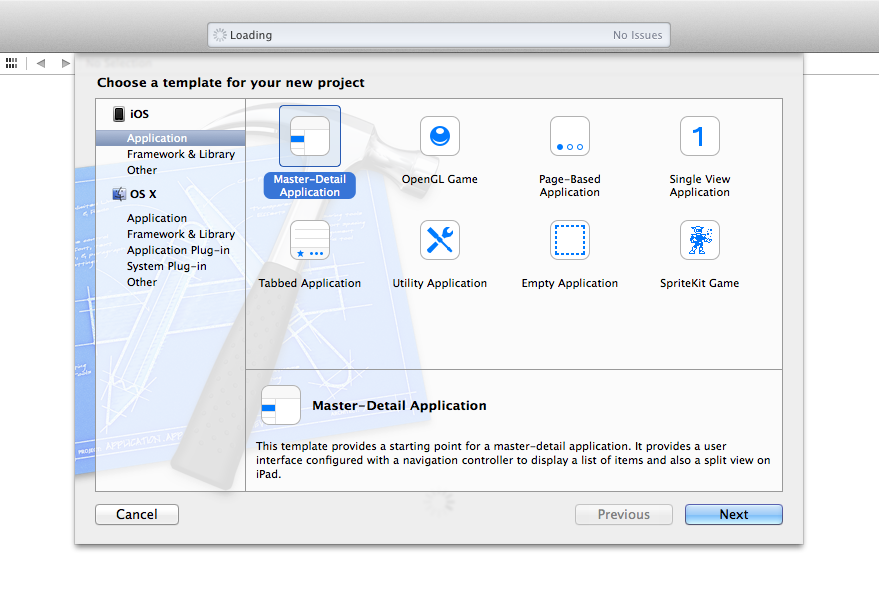
\includegraphics[scale=0.4]{xcode-templates}
	\caption{Auswahlbildschirm der verschiedenen Templates}
	\label{xcode-templates}
\end{figure}

Nach der Auswahl des Templates, werden die dem Template entsprechenden Dateien im Dateiexplorer angelegt.


Dazu gehören beispielsweise die \emph{AppDelegate} und die \emph{Storyboards}.

Die AppDelegate-Klasse steuert applikationsweite Ereignisse, wie etwa das Aufrufen und Schließen der Applikation. Außerdem wird durch die AppDelegate der aktuelle Zustand der Applikation gespeichert und bei Bedarf wiederhergestellt.


\textbf{Interface Builder}

Der Interface Builder ist ein in Xcode integrierter, grafischer Editor, welcher es erlaubt die Benutzeroberflächer einer iOS-Applikation zu erstellen. Dabei werden Storyboards genutzt.
Ein Storyboard ist die Repräsentation der grafischen Oberfläche einer Applikation und besteht dabei aus einem oder mehreren Views.

Die Views lassen sich nach dem \emph{Drag and Drop}-Prinzip zusammenstellen. Dabei stehen weitere Inteface-Elemente, wie zum Beispiel Textfelder, Buttons oder Schalter, zur Verfügung.

\begin{figure}[htb!]
	\centering
	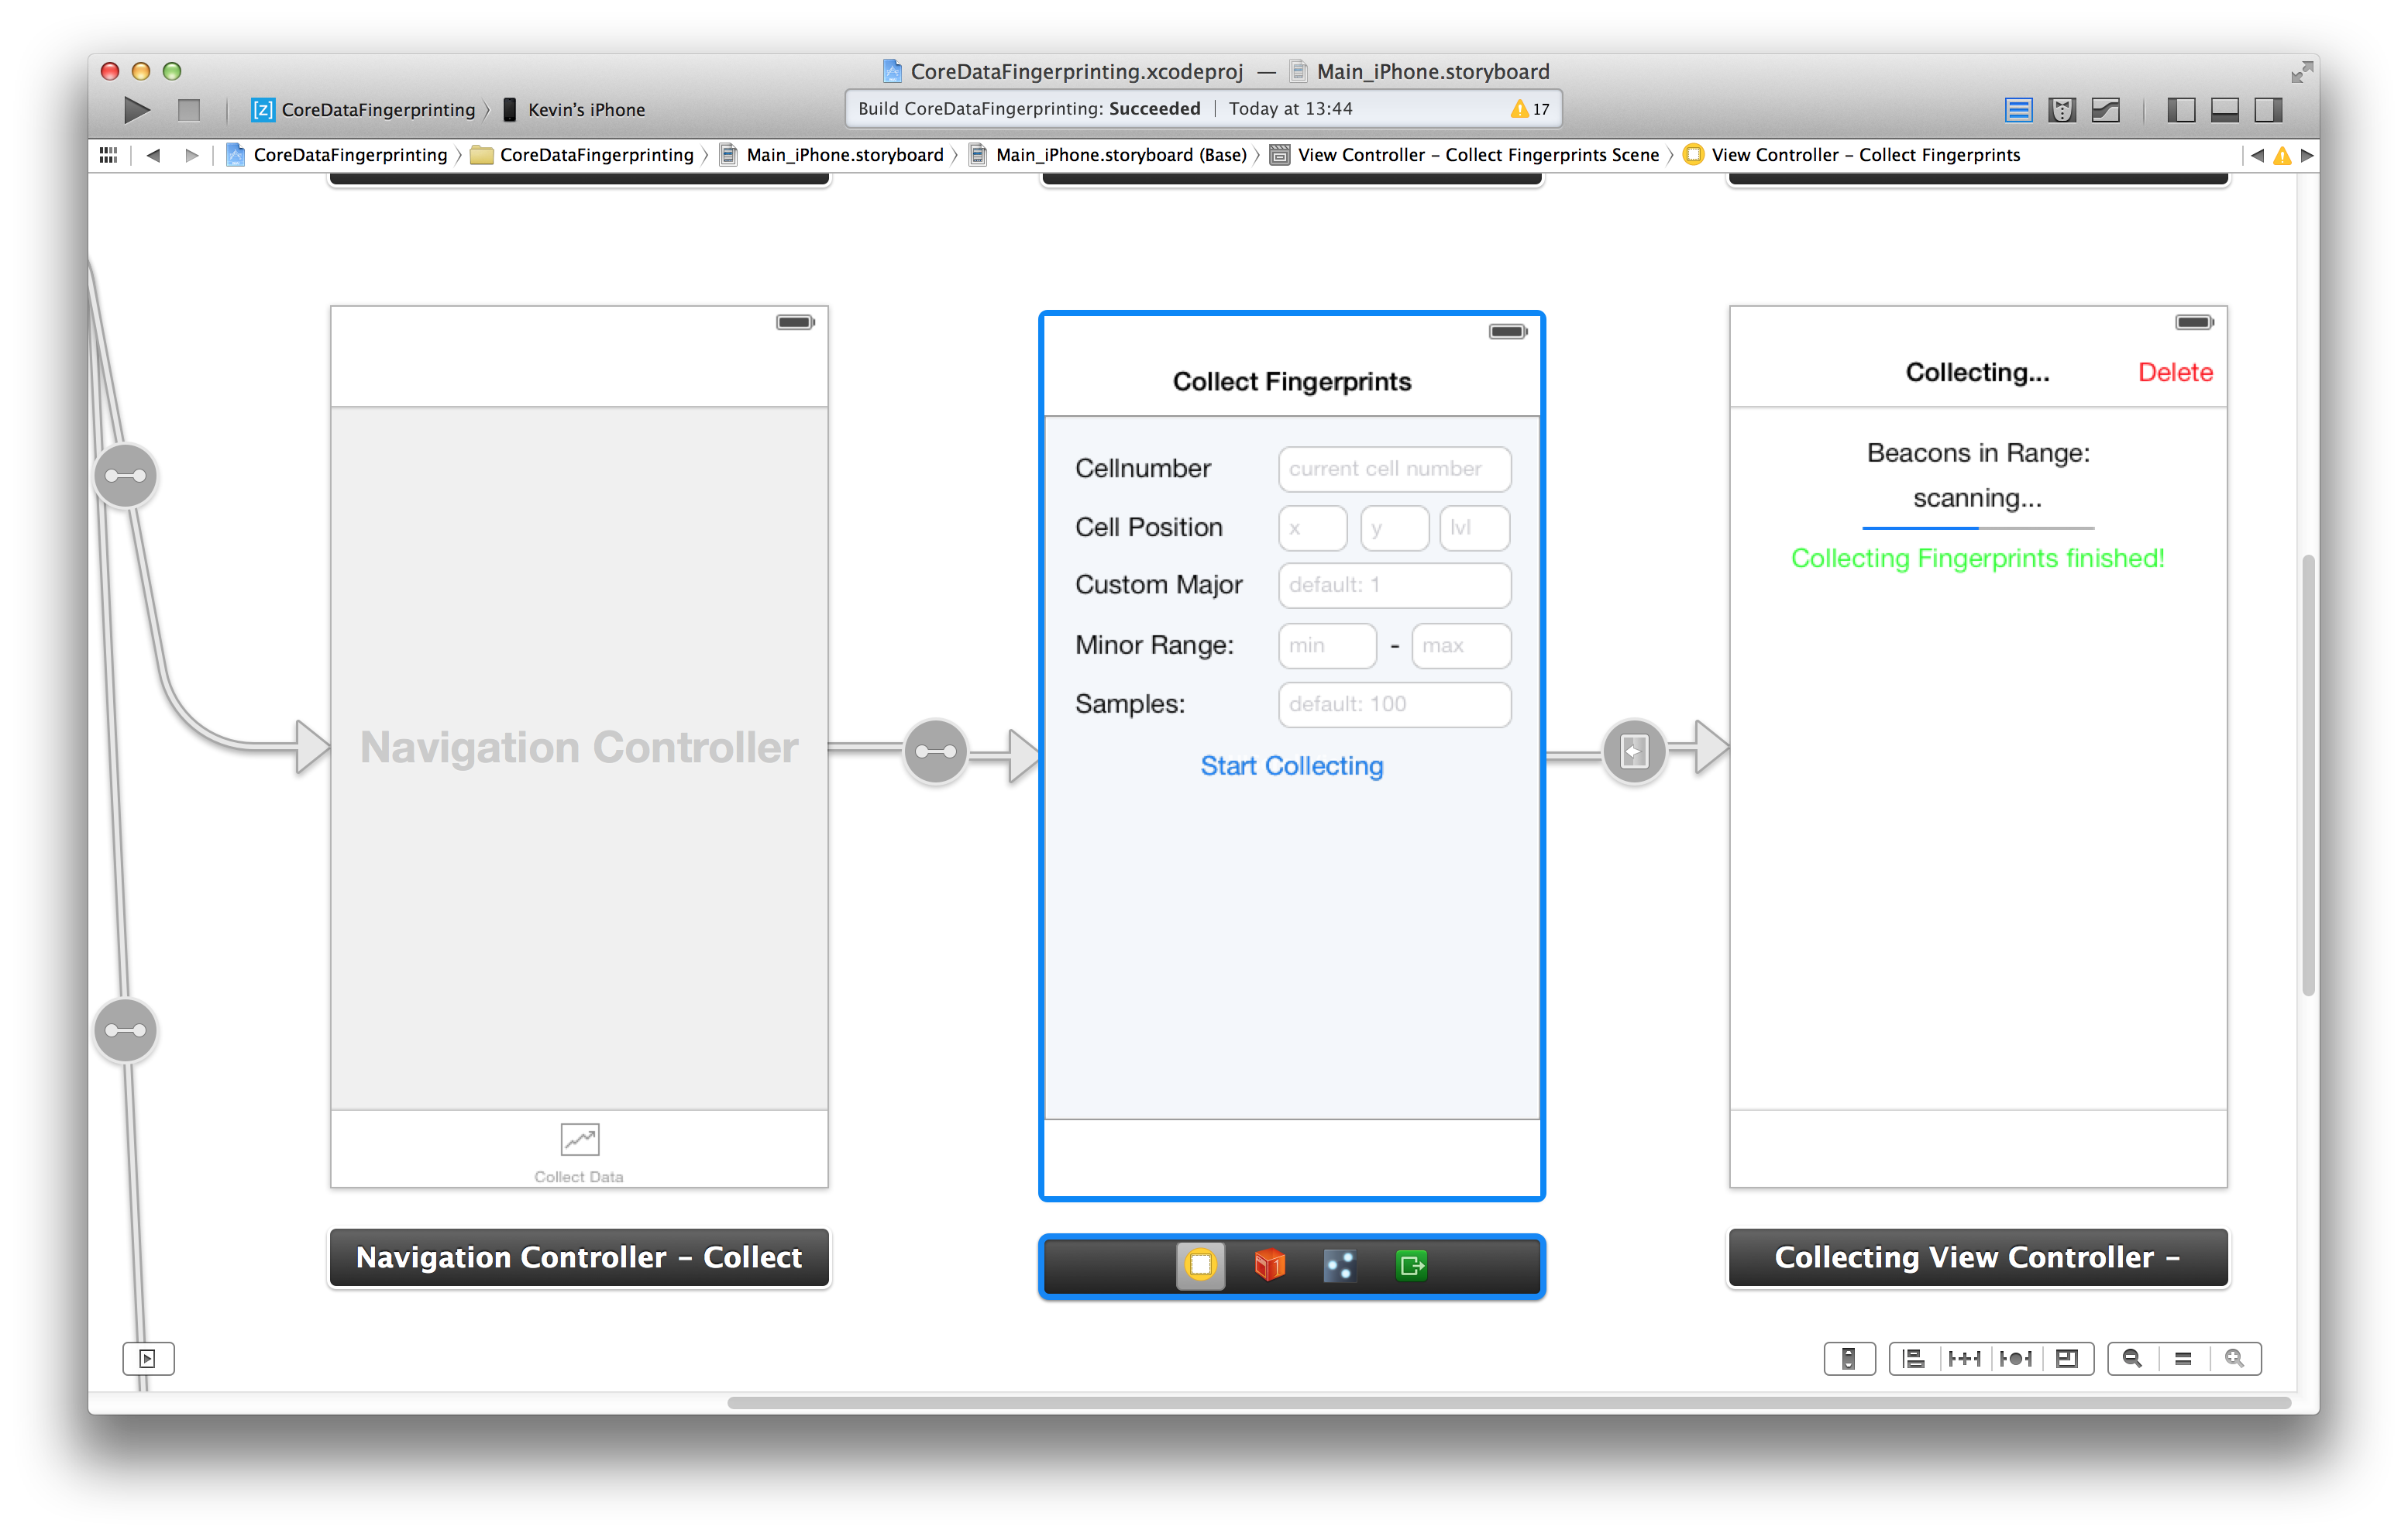
\includegraphics[scale=0.25]{xcode-storyboard}
	\caption{Interface Builder für eine iPhone-Applikation}
	\label{xcode-interface-builder}
\end{figure}

Wie in Abbildung \ref{xcode-interface-builder} zu erkennen, besteht das Storyboard aus mehreren Views, die jeweils eine gezeigte Szene auf dem Gerät repräsentieren. Die einzelnen Views sind mit \emph{Segue's} verbunden. Ein Segue, auf deutsch Übergang, steuert dabei den Wechsel zwischen den Views. Dabei wird zum Beispiel festgelegt durch welche Aktion dieser ausgelöst wird und wie dieser abläuft.


Der Interface Builder bietet außerdem noch die Funktion des \emph{Auto Layout}. Dabei werden sogenannte \emph{Constraints} genutzt, welche die Positionsbeziehungen zwischen den einzelnen Elementen des Views festlegen. Diese Constraints erzeugen so ein dynamisches Interface, welches sich an das verwendete Gerät anpasst und so ein User Interface, unabhängig der Bildschirmgröße oder der aktuellen Orientierung des Bildschirms, darstellt \cite{xcodeautolayout}.

\begin{figure}[htb!]
		\centering
	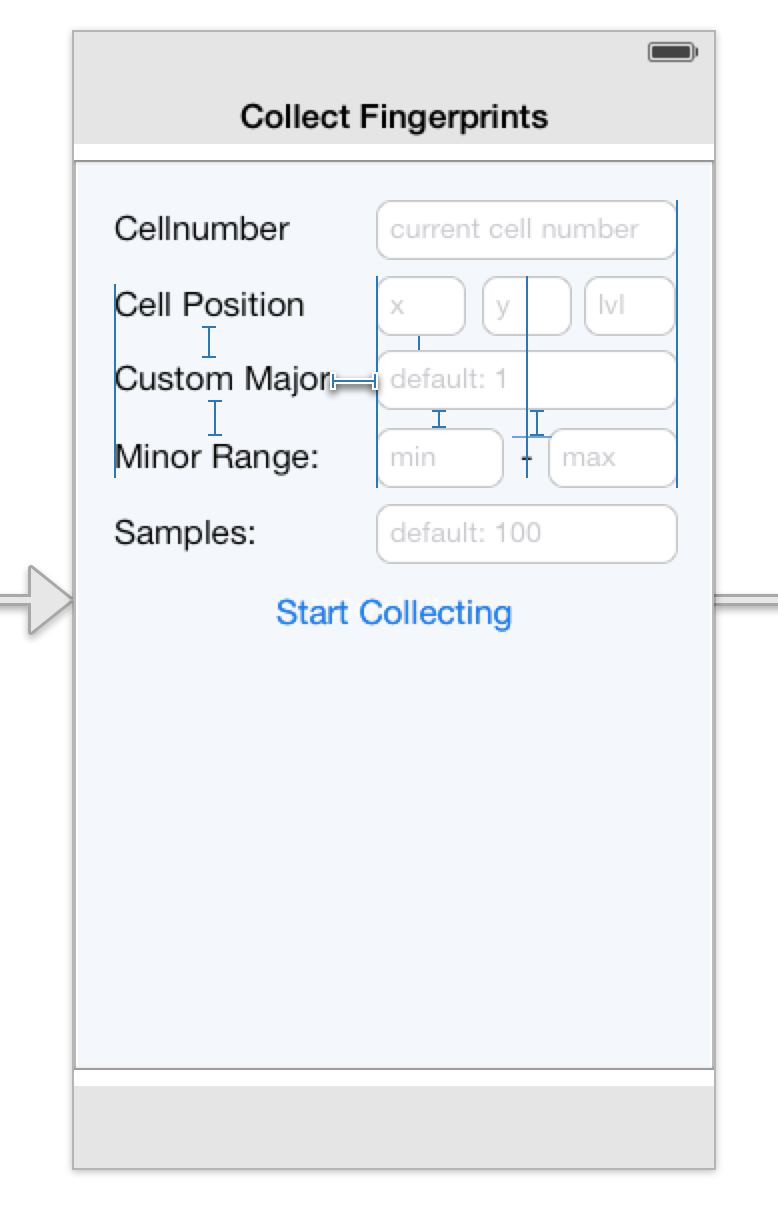
\includegraphics[scale=0.5]{xcode-storyboard-constraints}
	\caption{View Controller mit Constraints}
	\label{xcode-storyboard-constraints}
\end{figure}

Diese Constraints beschreiben dabei die Abstände und Ausrichtungen der einzelnen Elemente zu dem umschließenden View oder den Elementen innerhalb des Views.

Eine iOS-Applikation kann über mehrere Storyboards verfügen, wodurch es möglich ist, die gleiche Applikation sowohl für das iPhone als auch das iPad anzupassen.


\textbf{iOS Simulator}

Für das Testen und Debuggen der Applikation bringt Xcode einen iOS-Simulator mit sich. Dieser erlaubt das Ausführen einer Applikation auch ohne ein iPhone oder iPad. Der Simulator bietet dabei verschiedene Konfigurationen, sowohl für iPhone (3,5 Zoll und 4 Zoll) als auch für das iPad (retina und non-retina).
Im Bezug auf Bluetooth bietet der Simulator jedoch keine entsprechende Unterstützung \cite{iossimulator}.

%%%%%%%%%%%%%%%%%%%%%%%%%%%%%%%%%%%%%%%%%%%%%%%%%%%%%%%%%%%%
\section{iOS}
\label{sec:technologies:iosandxcode}
%%%%%%%%%%%%%%%%%%%%%%%%%%%%%%%%%%%%%%%%%%%%%%%%%%%%%%%%%%%%
Für die Entwicklung der Applikation zur Indoor Positionierung war eine der Vorgaben, dass diese für iOS programmiert werden soll.
Apple hat dabei für die iOS Programmierung verschiedene Vorraussetzungen. Zum einen benötgt man einen Mac, da nur hier die benötigte Software installiert werden kann.
Dazu zählt in erster Linie Xcode, welches als Entwicklungsumgebung für iOS-Applikationen genutzt wird \cite{iossetup}. 
Außerdem wird ein iOS-Gerät vorrausgesetzt, da, wie bereits erwähnt, der iOS-Simulator kein Unterstützung für Bluetooth mit sich bringt. 
Die eingesetzten iOS-Gerät sind ein iPhone 5 und ein iPhone 4s. Auf beiden Geräten ist die aktuelle iOS-Version 7.1 installiert.

Die vorrausgesetzte, minimale iOS-Version ist dabei iOS 7, da die iBeacon-API des CoreLocation-Frameworks (mehr dazu im Kapitel \ref{sec:technologies:corelocation}) erst ab dieser Version zur Verfügung stehen.

Die iOS-Applikationen basieren dabei auf dem Model-View-Controller Konzept. Dabei gibt es eine strenge Trennung zwischen den Daten, der Programmlogik und der Darstellung. 
Die Views in iOS sind dabei für die Darstellung der Daten und das Entgegennehmen von Nutzerinteraktionen zuständig. Die Programmlogik, welche die Daten bereitstellt und auf Nutzerinteraktionen reagiert, befindet sich dabei in einem ViewController. Für die Datenspeicherung stellt iOS verschiedene Möglickeiten zur Verfügung. Die am Häufigsten genutzten sind die \emph{Property Lists}, welche einer einfachen Textdatei mit vorgegebener Formatierung entsprechen, und CoreData, ein Speichermodell für iOS und OS X (siehe Kapitel \ref{sec:technologies:coredata}).

%%%%%%%%%%%%%%%%%%%%%%%%%%%%%%%%%%%%%%%%%%%%%%%%%%%%%%%%%%%%
\textbf{iOS Developer Program}
Um eine programmierte Anwendung letztendlich auf einem iOS-Gerät auszuführen, ist die Mitgliedschaft im iOS Developer Program notwendig.
Diese erlaubt das Testen der Anwendung auf dem Gerät, die Veröffentlichung im AppStore und gewährt Zugriff auf das iOS Beta-Programm, um Anwendungen für neue Versionen des Betriebssystems zu optimieren.
Die Mitgliedschaft in diesem \emph{iOS Developer Program} kostet jährlich 99 Dollar \cite{iosdevprog}. 
Im Rahmen meine Bachelorarbeit wurde der Zugang zu diesem Programm von der Universität zur Verfügung gestellt. Dabei beschränkt sich der Funktionsumfang jedoch auf das Testen der Applikation auf dem Gerät, da die Veröffentlichung im AppStore und der iOS Beta-Programm nicht teil des Pakets für Universitäten ist.

\textbf{iPhone}
Für die Entwicklung und das Testen der Applikation wurde ein iPhone 5 und ein iPhone 4s verwendet. 
Hauptsächlich wurde das iPhone 5 genutzt, wobei das iPhone 4s als Vergleichsgerät diente, um Messwerte zu vergleichen oder zu überprüfen.

Das Ausführen der geplanten Applikation auf einem realen Endgerät ist dabei unverzichtbar, da der iOS-Simulator nicht die Möglichkeit besitzt Bluetooth-Signale zu empfangen.

Das iPhone 4s wurde dazu genutzt, zu überprüfen in wie weit die Ergebnisse der Messwert zwischen einzelnen Geräten übertragbar sind, beziehungsweise wie sich diese zwischen einzelnen Modellgenerationen unterscheiden, da diese verschiedene Hardware einsetzen. 

So setzt das iPhone 4s auf den Broadcom BCM4330-Chipsatz, welches ein Wireless LAN-Chip mit integriertem Bluetooth 4.0 ist \cite{iPhone4sTeardown}. Das iPhone 5 dagegen setzt auf den BCM4334 \cite{iPhone5Teardown}, ebenfalls von Broadcom. 
Auch der Aufbau der Antennen und das Material der iPhones unterscheidet sich zwischen diesen beiden Generationen deutlich. 
So ist das iPhone 4s mit einer Glas-Rückseite ausgestattet, wohingegen das iPhone 5 einen Rückseite aus Aluminium besitzt.

Daher ist es wichtig zu vergleichen, in wie weit diese Unterschiede Einfluss auf die Empfangsqualität haben und zu bestimmen, ob eine Übertragung der Messwerte zwischen den Geräten möglich ist oder jedes Gerät individuell behandelt werden muss.

\begin{figure}[htb!]
		\centering
	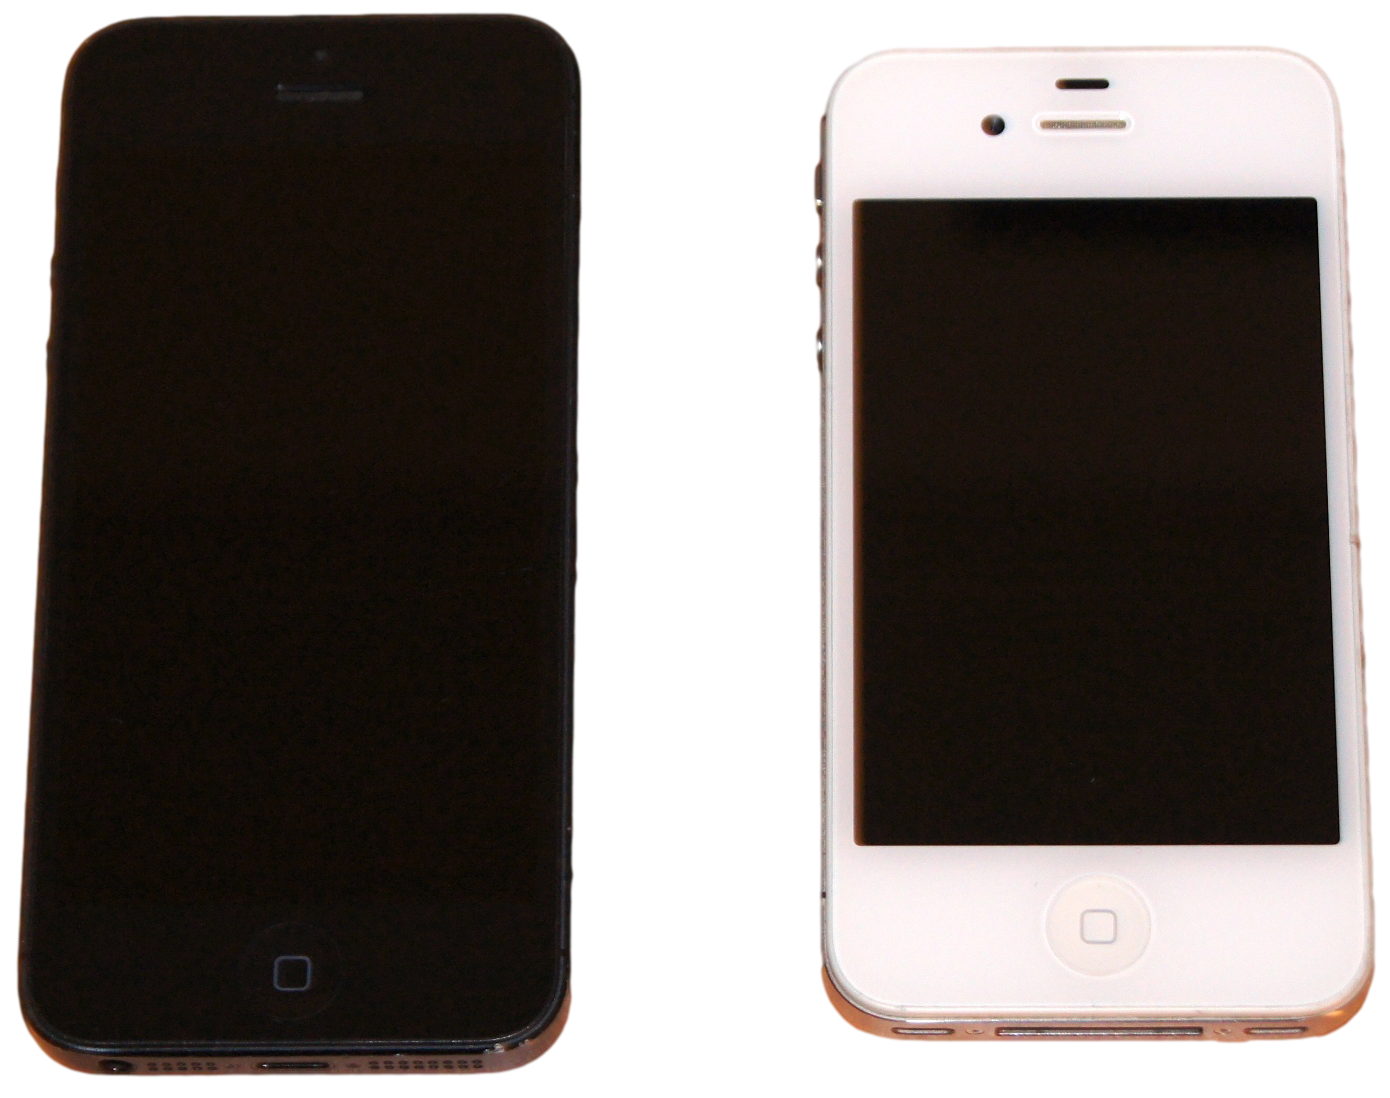
\includegraphics[scale=0.1]{iphones}
	\caption{Die für die Messungen und Tests genutzten iPhones}
	\label{iphones}
\end{figure}

\textbf{Objective-C}
Für die Implementierung der Applikation kam als Programmiersprache \emph{Objective-C} zum Einsatz, welches die primäre Sprache zur Programmierung von iOS-Anwendugen ist. 
Diese bietet viele nützliche Eigenschaften, wie etwa dynamisches Binden, eine dynamische Typisierung oder \emph{Fast Enumeration}.
Im Vergleich zu Java arbeitet \emph{Objective-C} nicht mit Methodenaufrufen, sondern mit Nachrichten. Diese werden von einem Sender zu einem Empfänger gesendet, wobei der Empfänger daraufhin entscheidet, was geschieht beziehungsweise welche Methode ausgeführt wird. Ein weitere Besonderheit von Objective-C sind die Properties (Eigenschaften), welche den Instanzvariablen entsprechen, jedoch noch weitere Konfigurationsmöglichkeiten hinsichtlich Schreibschutz und Atomarität bieten.
Eine weiterer Unterschied ist die Syntax von Objective-C.

\begin{listing}[htb!]
    \insertminted{objc}{code_examples/helloworld.m}
    \caption{Hello World-Beispiel in Objective-C und Java}
	\label{lst:helloworld_objc}
\end{listing}

Der Hauptunterschied liegt in der Methodendeklaration. Statt des \emph{static} Schlüsselwortes wird bei Objective-C eine Klassenmethode mit einem ''+'' gekennzeichnet. Eine Instanzmethode wird mit einem ''-'' deklariert. Der nächste Unterschied wird bei den Übergabewerten deutlich. Diese werden bei Objective-C, mit einem '':'' abgetrennt, angegeben.
Ein weiterer Unterschied wird beim Aufruf der Methoden deutlich. Da Objective-C nicht explizit die Methode aufruft, sondern eine Nachricht an die Klasse sendet, unterscheidet sich die Syntax deutlich. So werden hier eckige Klammern genutzt, wobei der Empfänger der Nachricht zuerst aufgeführt wird und danach die zu sendende Nachricht eingefügt wird \cite{objc}).


%%%%%%%%%%%%%%%%%%%%%%%%%%%%%%%%%%%%%%%%%%%%%%%%%%%%%%%%%%%%
\section{CoreLocation-Framework}
\label{sec:technologies:corelocation}
%%%%%%%%%%%%%%%%%%%%%%%%%%%%%%%%%%%%%%%%%%%%%%%%%%%%%%%%%%%%
Das CoreLocation-Framework ist ein iOS-Framework, welches es erlaubt die aktuellen Positions- und Richtungsinformationen eines Gerätes zu bestimmen und auszugeben.
Die Positionsbestimmung lässt sich dabei über verschiedene Sensoren und Werte bestimmen, wobei der Grad der Genauigkeit variabel ist.
Für die Positionsbestimmung lässt sich zum Beispiel das integrierte GPS-Modul verwenden.
Auch die Aktualisierungsrate der Position lässt sich festlegen, wobei eine höhere Aktualisierungsrate und eine höhere Genauigkeit auch gleichbedeutend mit einem höherem Akkuverbrauch sind.
	
Die Genauigkeit lässt sich dabei nur bei der Positionierung mittels GPS einstellen und ist daher für die Indoor Positionierung nur bedingt geeignet. Es wäre jedoch denkbar, die Positionierung mittels GPS und die Positionierung mittels iBeacons zu verbinden und nahtlos in einander übergehen zu lassen.

Eine weitere Funktion des CoreLocation-Frameworks ist der Kompass, also die Bestimmung der Himmelsrichtungen. Durch den eingebauten Kompass in den neueren iOS-Geräten ist es möglich, die aktuelle Ausrichtung des Gerätes sehr genau zu bestimmen. Dies ist im Bezug auf die Indoor Navigation hilfreich, da diese Informationen in die Positionsbestimmung einbezogen werden können. Da der menschliche Körper die Signale der Beacons beeinflusst, ist es daher von Vorteil die aktuelle Ausrichtung zu kennen. Dadurch kann die aktuelle Position des Körpers bestimmt werden und in den Messungen berücksichtigt werden.

Des Weiteren erlaubt diese Funktion eine dynamische Anpassung der Karte, abhängig davon wie das Gerät aktuell ausgerichtet ist.

Die für uns zentrale Funktion dieses Frameworks ist die Erkennung von iBeacons und die Funktionen zur Verarbeitung der von den Beacons gesendeten Daten.
Mittels des Frameworks können Beacons anhand ihres UUID erkannt und einer Region zugeordnet werden. Die genaue Funktionsweise wird dabei im folgenden Kapitel behandelt \cite{corelocation}.

%%%%%%%%%%%%%%%%%%%%%%%%%%%%%%%%%%%%%%%%%%%%%%%%%%%%%%%%%%%%
\subsection{iBeacons-API}
\label{sec:technologies:corelocation:ibeaconsapi}
%%%%%%%%%%%%%%%%%%%%%%%%%%%%%%%%%%%%%%%%%%%%%%%%%%%%%%%%%%%%
Mit der iOS Version 7 wurde das CoreLocation Framework um die Beacon-Funktionalitäten erweitert. 
Dazu wurden zwei neue Klassen hinzugefügt und das bestehende Framework dementsprechend angepasst. 
Hinzugefügt wurde zum einen die \emph{CLBeacon}-Klasse \cite{clbeaconref}, welche ein iBeacon repräsentiert und alle zur verfügungsteheneden Informationen enthält und zum anderen die \emph{CLBeaconRegion}-Klasse \cite{clbeaconregionref}, welche eine Region mit mehreren Beacons, abhängig von ihrem UUID und weiteren Werten, beschreibt.

Die \emph{CLBeacon}-Klasse besteht dabei lediglich aus Properties mit den gegebenen Beacon-Informationen, wie \emph{UUID}, \emph{major}, \emph{minor}, \emph{accuracy}, \emph{proximity} und \emph{rssi}.

Die \emph{CLBeaconRegion}-Klasse ist etwas umfangreicher und bestimmt letztendlich, nach welchen Beacons gesucht werden soll.
Dabei ist es möglich die Region in verschiedene Genaugikeits-Stufen zu initialisieren:


\emph{initWithProximityUUID:identifier:}\begin{quote}
	Die Region ist nur abhängig von dem UUID und dem Identifier der Beacons, das heißt es werden alle Beacons mit dem gegebenen UUID gesucht.
\end{quote}
\emph{initWithProximityUUID:major:identifier:}\begin{quote}
	Die Region ist abhängig von dem UUID, dem Identifier und dem Major-Wert der Beacons. Es werden nur Beacons eines bestimmten Major-Wertes gesucht.
\end{quote}
\emph{initWithProximityUUID:major:minor:identifier:}\begin{quote}
	Die Region ist abhängig von dem UUID, dem Identifier, dem Major-Wert und dem Minor-Wert der Beacons. Es werden nur Beacons mit passendem Major und Minor-Wert gesucht. In diesem Fall ist bei mehreren erkannten Beacons keine Unterscheidung mehr möglich.
\end{quote}

Die Beacon-Region bestimmt also letztlich nach welchen Beacons gesucht wird, beziehungsweise welche Beacons gefunden werden.

%%%%%%%%%%%%%%%%%%%%%%%%%%%%%%%%%%%%%%%%%%%%%%%%%%%%%%%%%%%%
\section{Mapbox}
\label{sec:sec:technologies:mapbox}
%%%%%%%%%%%%%%%%%%%%%%%%%%%%%%%%%%%%%%%%%%%%%%%%%%%%%%%%%%%%
MapBox ist ein Online-Landkarten Anbieter, welcher es erlaubt eigene Karten zu erstellen und über ihren Service online bereitzustellen \cite{mapboxweb}. 
Die Grundkarten werden dabei aus dem OpenStreetMap-Projekt entnommen und Mapbox erlaubt es diese Karten grafisch zu überarbeiten, um so zum Beispiel das Farbschema zu ändern, eigene Markierungen hinzuzufügen oder auch eigene Layer über die Karte zu legen.

Außerdem stellt Mapbox ein SDK \cite{mapboxsdk} für iOS bereit, welche es erlaubt diese individuell angepassten Karten in iOS anzuzeigen und gleichzeitig die Funktionen des native MapKit-Framework, wie zum Beispiel Pinch-to-Zoom, automatische Kompassausrichtung oder Annotationen auf der Karte, mit sich bringt. Zudem besitzt Mapbox eine größere Flexibilität im Bezug auf die individuelle Anpassung der Karten und den Offline-Betrieb, als das von Apple für iOS bereitgestellte MapKit-Framework. Das Mapbox-SDK erlaubt es zum Beispiel die Karten direkt auf dem Gerät zu speichern.

Bisher ist die Unterstützung von Indoor-Karten jedoch noch nicht gegeben, sodass hierbei nicht auf vorhandenes Kartenmaterial zurückgegriffen werden kann, sondern eigenes Kartenmaterial bereitstellen muss.

Google hat mit \emph{Google Maps Indoor} bereits einen Dienst gestartet, welcher Gebäudepläne in Google Maps integriert (siehe \cite{googleindoormaps}. Dabei handelt es sich bisher jedoch hauptsächlich um öffentliche Gebäude in US-amerikanischen Städten. In Deutschland ist der Dienst ebenfalls schon gestartet, beinhaltet jedoch nur wenige Gebäude. Das Hinzufügen von neuen Gebäudeplänen ist nur bei öffentlichen Gebäuden möglich und nicht für den privaten Gebrauch vorgesehen, daher konnte nicht auf diesen Dienst zurückgegriffen werden.

Die Indoor-Karten mussten daher individuell für den Einsatzort erstellt und in ein, von Mapbox verständliches Format, umgewandelt werden.
Die Ausgangsdatei ist dabei eine Bilddatei in JPEG-Format, welches eine Karte des Innenraumes zeigt. Dieses Datei muss zur weiteren Verwendung in ein von Mapbox verständliches Format umgewandelt werden. 
Dazu wurde ein von ''Tom MacWright'' \cite{jpgtogeo} bereitgestellte Python-Script verwendet, welches JPEG Dateien in GeoTIFF Dateien umwandelt. Die GeoTIFF-Datei \cite{geotiff} speichert neben den eigentlichen Bildinformationen zusätzlich Koordinaten für die Georeferenzierung. 

Mit dieser GeoTIFF-Datei ist es nun möglich eine eigene Karte zu erstellen, welche letztendlich auf dem iOS-Gerät ausgegeben wird.
Dafür stellt Mapbox das Programm \emph{TileMill} zur Verfügung \cite{tilemill}. Dieses erlaubt es eigene Karten zu erstellen und zu bearbeitet. Die erstellte Karte kann anschließend in verschiedenen Formaten exportiert werden. 
TileMill bietet einen Import von GeoTIFF-Dateien an, sodass unsere Karte direkt eingefügt werden kann.

\begin{figure}[htb!]
	\centering
	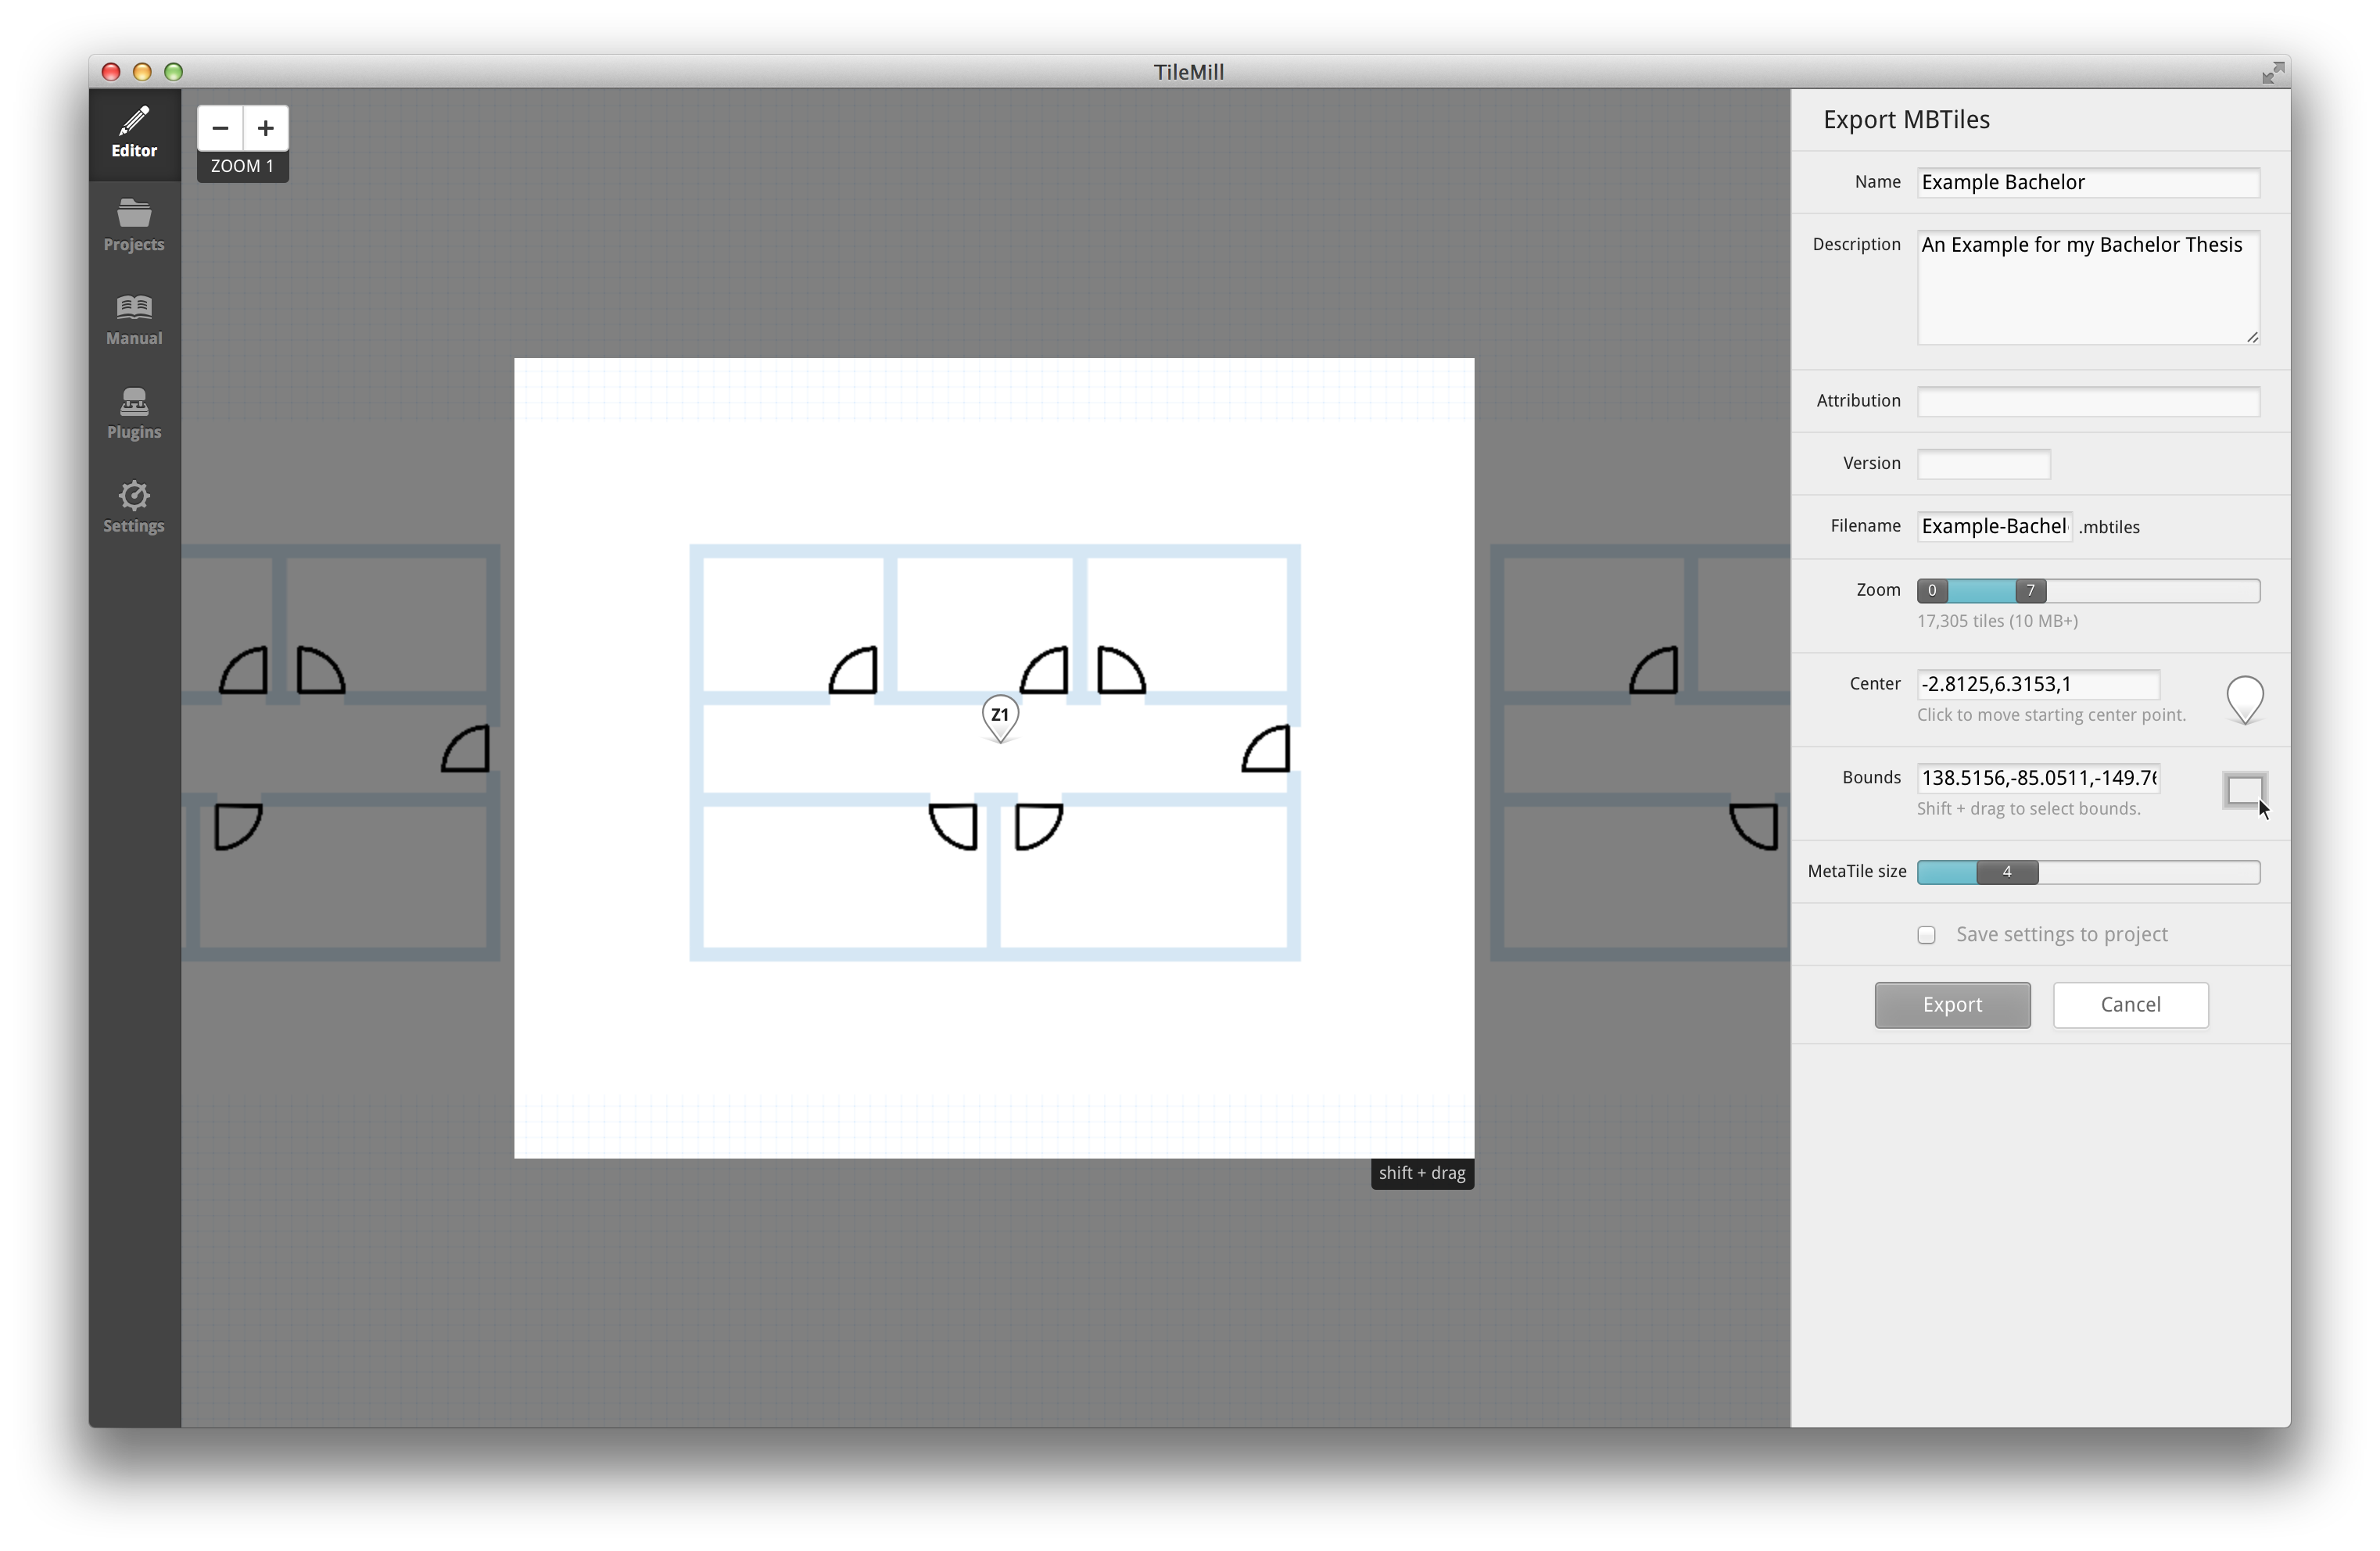
\includegraphics[scale=0.25]{tilemill-example}
	\caption{Karte in TileMill}
	\label{tilemill-example}
\end{figure}

TileMill erlaubt es nun die eingefügte Karte weiter zu bearbeiten oder Informationen hinzuzufügen.
Der nächste Schritt ist es die Karte in ein für iOS beziehungsweise das Mapbox SDK, verständliches Format zu überführen.
Dazu wird die Karte im \emph{mbtiles}-Format exportiert \cite{mbtiles}. Dies ist ein von Mapbox entwickeltes Dateiformat, welches die Karte in einzelne Kacheln überführt und speichert. Dadurch wird das Laden der einzelnen Kartenabschnitte bei größeren Karten beschleunigt, da nicht die komplette Karte geladen werden muss, sondern nur die aktuell benötigten Kacheln.

Die erzeugte \emph{.mbtiles}-Datei lässt sich nun in die iOS Applikation einbinden und über das SDK auf dem iOS-Gerät ausgeben. In Abbildung \ref{mapbox-map-ios} sieht man die Ausgabe einer Karte auf dem iPhone 5.

\begin{figure}[htb!]
		\centering
	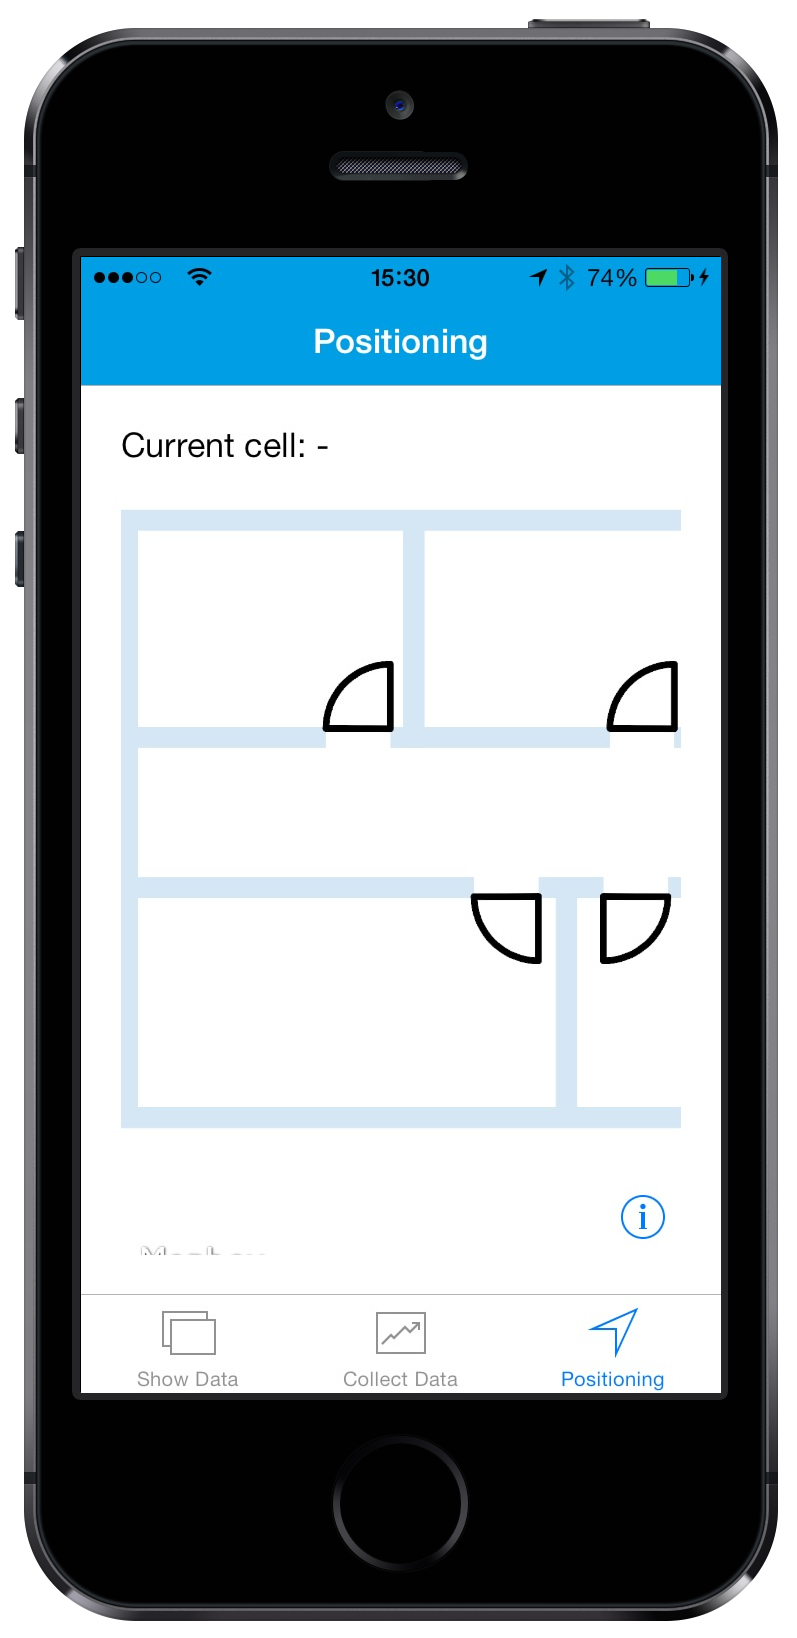
\includegraphics[scale=0.25]{mapbox-map-ios-mockup}
	\caption{Kartenausgabe mittels Mapbox SDK auf dem iPhone}
	\label{mapbox-map-ios}
\end{figure}

Diese Karte wird offline auf dem Gerät gespeichert, sodass keine Internetverbindung für die Anzeige nötig ist.

%%%%%%%%%%%%%%%%%%%%%%%%%%%%%%%%%%%%%%%%%%%%%%%%%%%%%%%%%%%%
\section{CoreData-Framework}
\label{sec:technologies:coredata}
%%%%%%%%%%%%%%%%%%%%%%%%%%%%%%%%%%%%%%%%%%%%%%%%%%%%%%%%%%%%
Das CoreData-Framework erlaubt die Verwaltung von Datenobjekten und deren Speicherung auf dem Gerät.
Dabei kommt ein relationales Datenmodell zum Einsatz, welches sich mittels grafischer Oberfläche in Xcode erstellen lässt.
In dem Modell lassen sich sowohl die Entitäten und ihre Attribute einstellen, als auch die Beziehungen zwischen den Entitäten definieren.
Die eigentliche Datenspeicherung sieht dabei drei verschiedene Speichermöglichkeiten vor: als Binärdatei, als XML-Datei oder in einer SQLite-Datenbank. 

Für die Erstellung eines CoreData-Modells bietet Xcode einen eigenen Editor an, welcher es erlaubt, Entitäten zum Modell hinzuzufügen und deren Attribute anzupassen. Die Beziehungen der Entitäten lassen sich dort ebenfalls erstellen und bearbeiten. Das Modell lässt sich dabei sowohl grafisch als auch in Tabellenform anzeigen.

\begin{figure}[htb!]
		\centering
	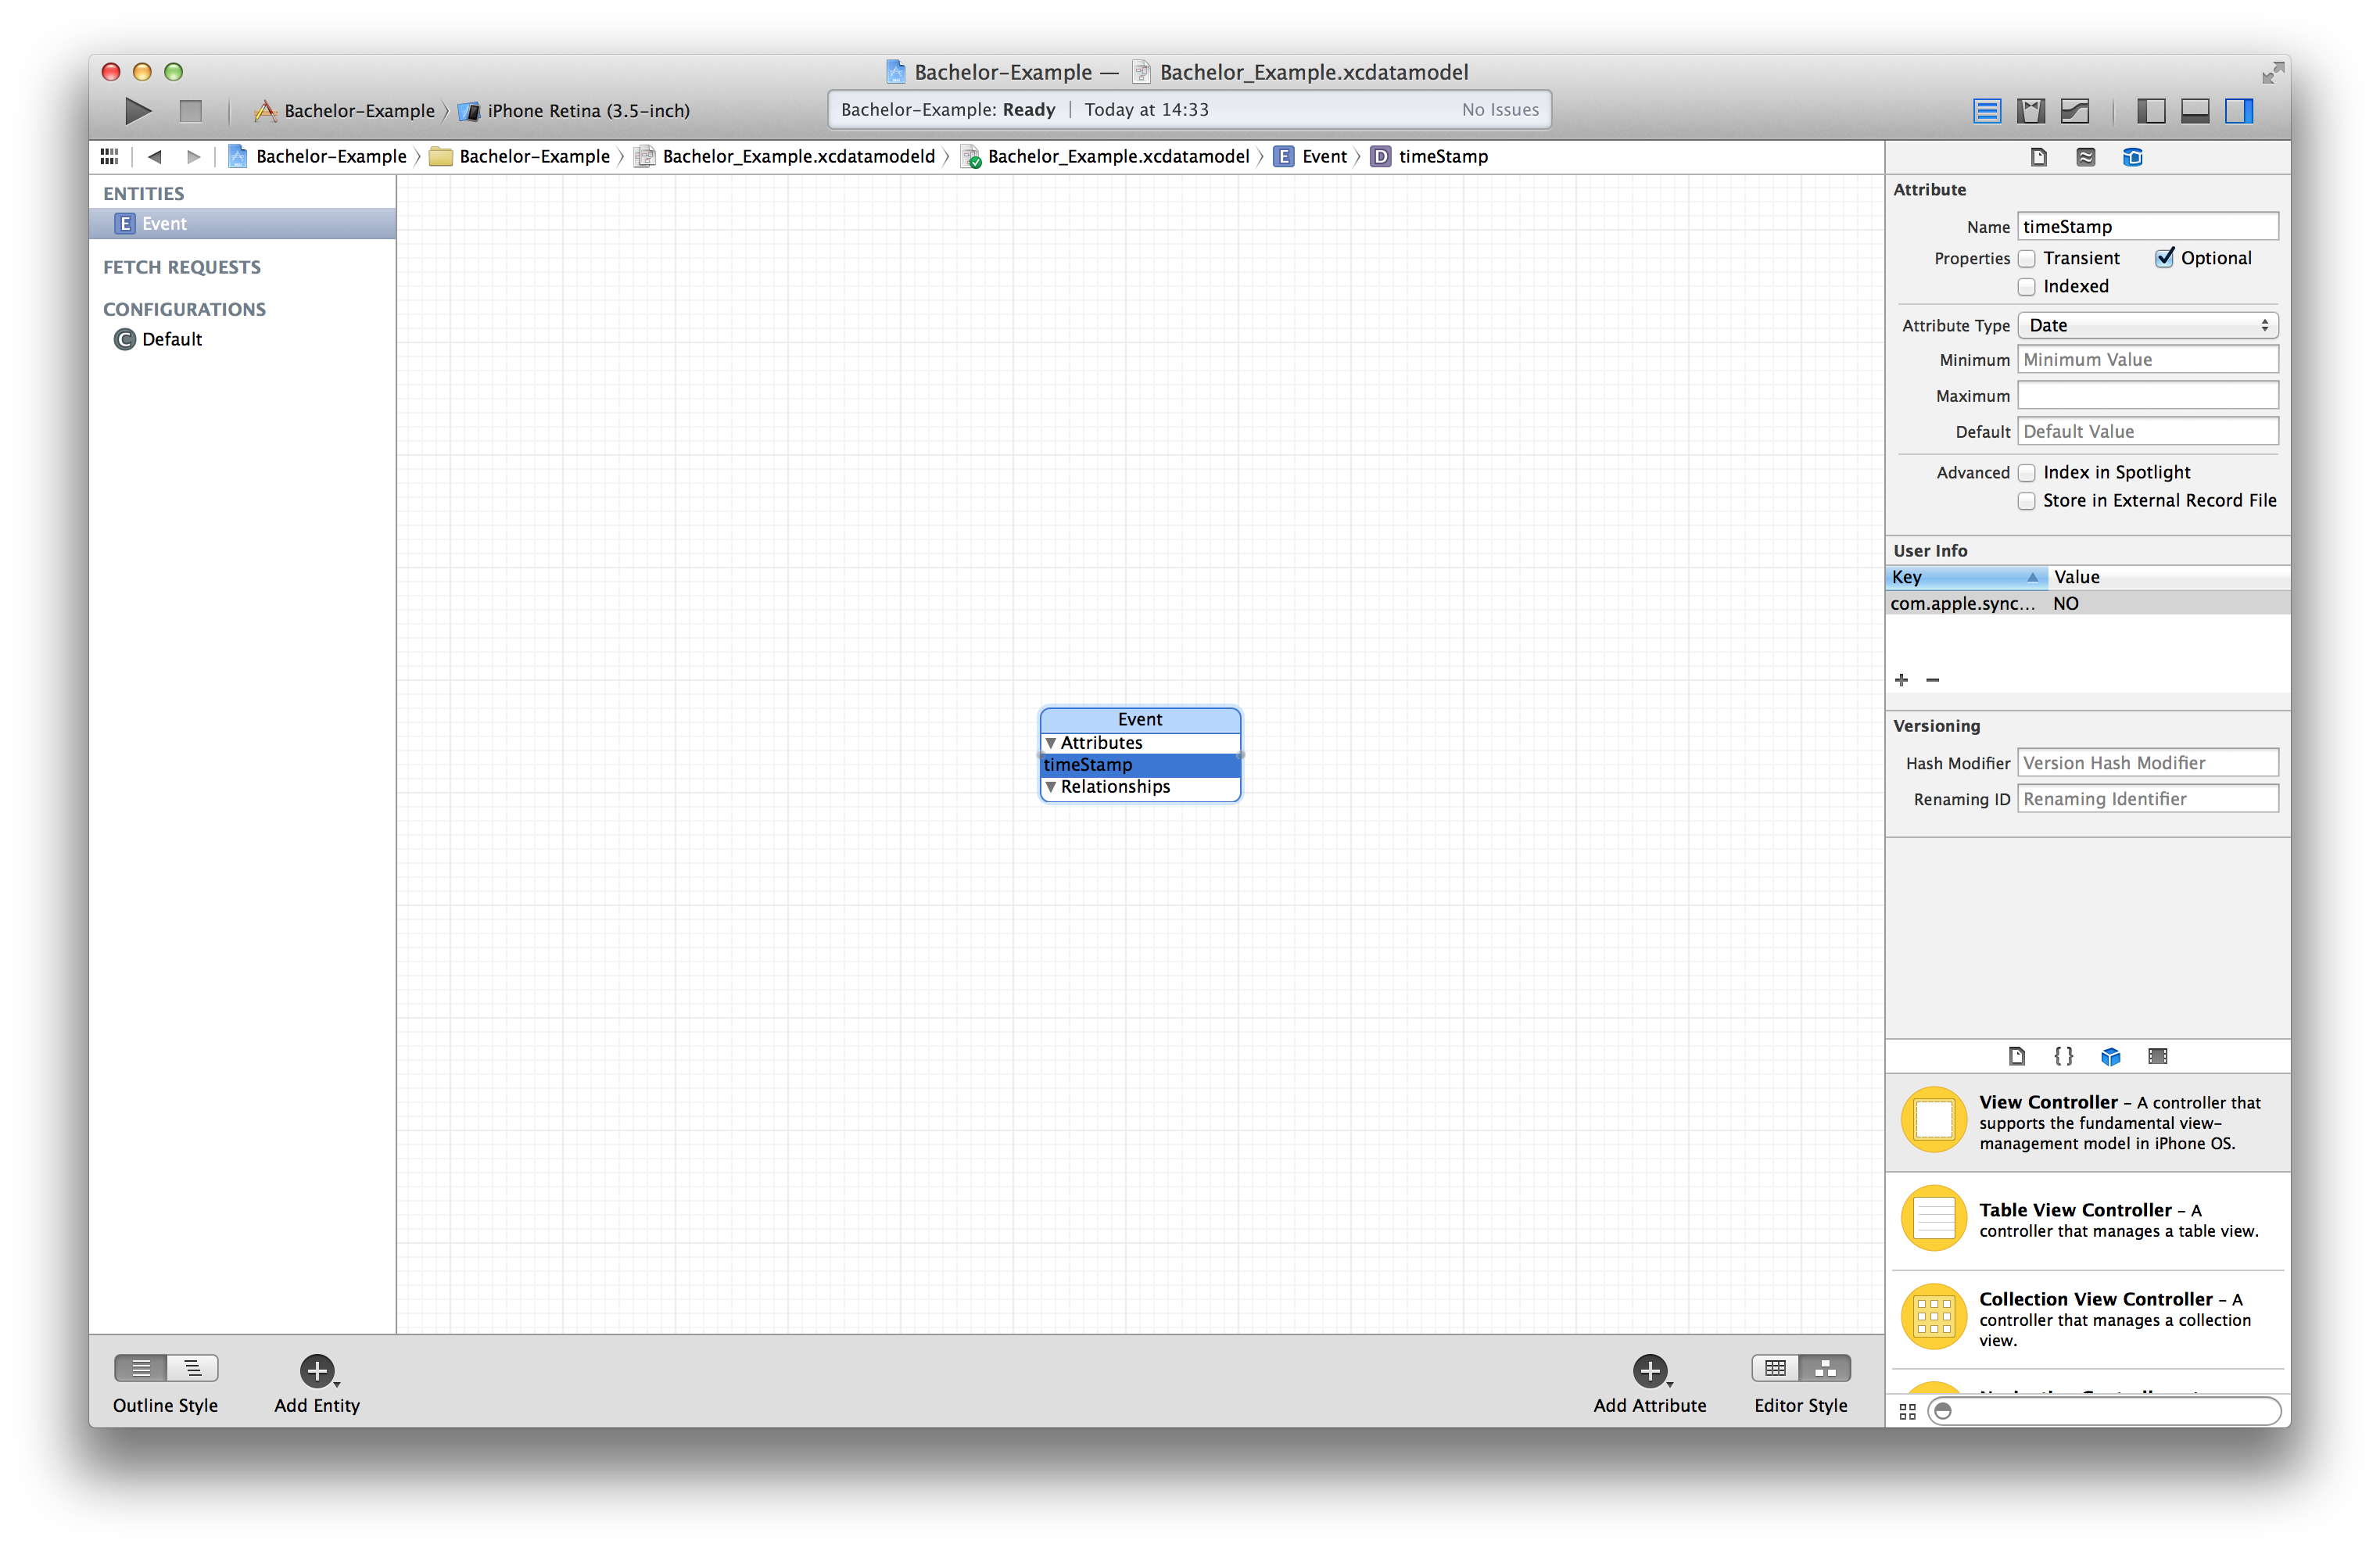
\includegraphics[scale=0.3]{coredata-editor}
	\caption{CoreData-Editor in der grafischen Darstellung.}
	\label{coredata-model}
\end{figure}


Nachdem ein CoreData-Modell konfiguriert wurde, benötigt man für den Zugriff auf das Modell ein \emph{NSManagedObjectContext}-Objekt, ein \emph{NSPersistentStoreCoordinator}-Objekt und ein \emph{NSManagedObjectModel}-Objekt. Das \emph{NSManagedObjectContext}-Objekt, verwaltet dabei alle Datenobjekte des Modells. Die Objekte sind dabei vom generischen Typ \emph{NSManagedObject}. Über den \emph{NSManagedObjectContext} werden neue Objekte zum Datenmodell hinzugefügt oder vorhandene Onjekte ausgelesen.

Nach dem Anlegen des Datenmodells ist es auch möglich, automatisiert eigene Klassen für die einzelnen Entitäten erzeugen zu lassen. Dabei wird für jede Entität eine entsprechende Klasse mit deren Attributen, in Form von Properties, angelegt. Dies erleichtert den Zugriff auf die einzelnen Attribute der Datenobjekte.

Um auf die Daten zuzugreifen und diese zu verändern ist es zunächst nötig sie aus der Datenbank zu extrahieren. Dazu verwendet man einen \emph{NSFetchRequest}, welcher Objekte nach bestimmten Kriterien aus der Datenmodell ausliest.
Dabei ist es möglich den \emph{NSFetchRequest} genauer zu spezifizieren und so nur Objekte mit bestimmten Eigenschaften auszulesen.
Dafür verwendet man ein \emph{NSPredicate}, welches umfangreiche Tests auf bestimmte Attribute und logische Operationen erlaubt.

\begin{listing}[htb! breaklines=true]
    \insertminted{objc}{code_examples/NSFetchRequest.m}
    \caption{Fetch Request für alle Objekte die mit Nachnamen ''Meier'' heißen und mehr als 3000 Euro im Monat verdienen}
	\label{lst:NSFetchRequest_objc}
\end{listing}

Als Rückgabewert erhält man ein Array mit allen Objekten, auf die die gegebenen Kriterien zutreffen.

Die Attribute dieser Objekte können nun ausgelesen und verändert werden. Um Veränderungen auch im Datenmodell zu übernehmen, muss lediglich der \emph{save}-Befehl des \emph{NSManagedObjectContext} ausgeführt werden \cite{coredataguide}.

%%%%%%%%%%%%%%%%%%%%%%%%%%%%%%%%%%%%%%%%%%%%%%%%%%%%%%%%%%%%
\section{Versionsverwaltung mit Git}
\label{sec:tools:git}
%%%%%%%%%%%%%%%%%%%%%%%%%%%%%%%%%%%%%%%%%%%%%%%%%%%%%%%%%%%%
Für die Verwaltung und Versionierung des Projektes wurde Git verwendet. Als Hosting-Plattform wurde dabei GitHub \cite{github} genutzt.

Git wurde gewählt, da es schnell und vergleichsweise einfach zu bedienen ist. Des Weiteren bietet Xcode bereits standardmäßig Git-Unterstützung mit einem grafischen Interface, welches alle nötigen Befehle wie Commit, Push, Pull oder die Erstellung eines neuen Branches auf Knopfdruck beherscht.

Auch ein Diff-Editor ist integriert, welcher es erlaubt die Unterschiede im Quelltext, zwischen verschiedenen Versionen zu begutachten.

\begin{figure}[htb!]
		  \centering
	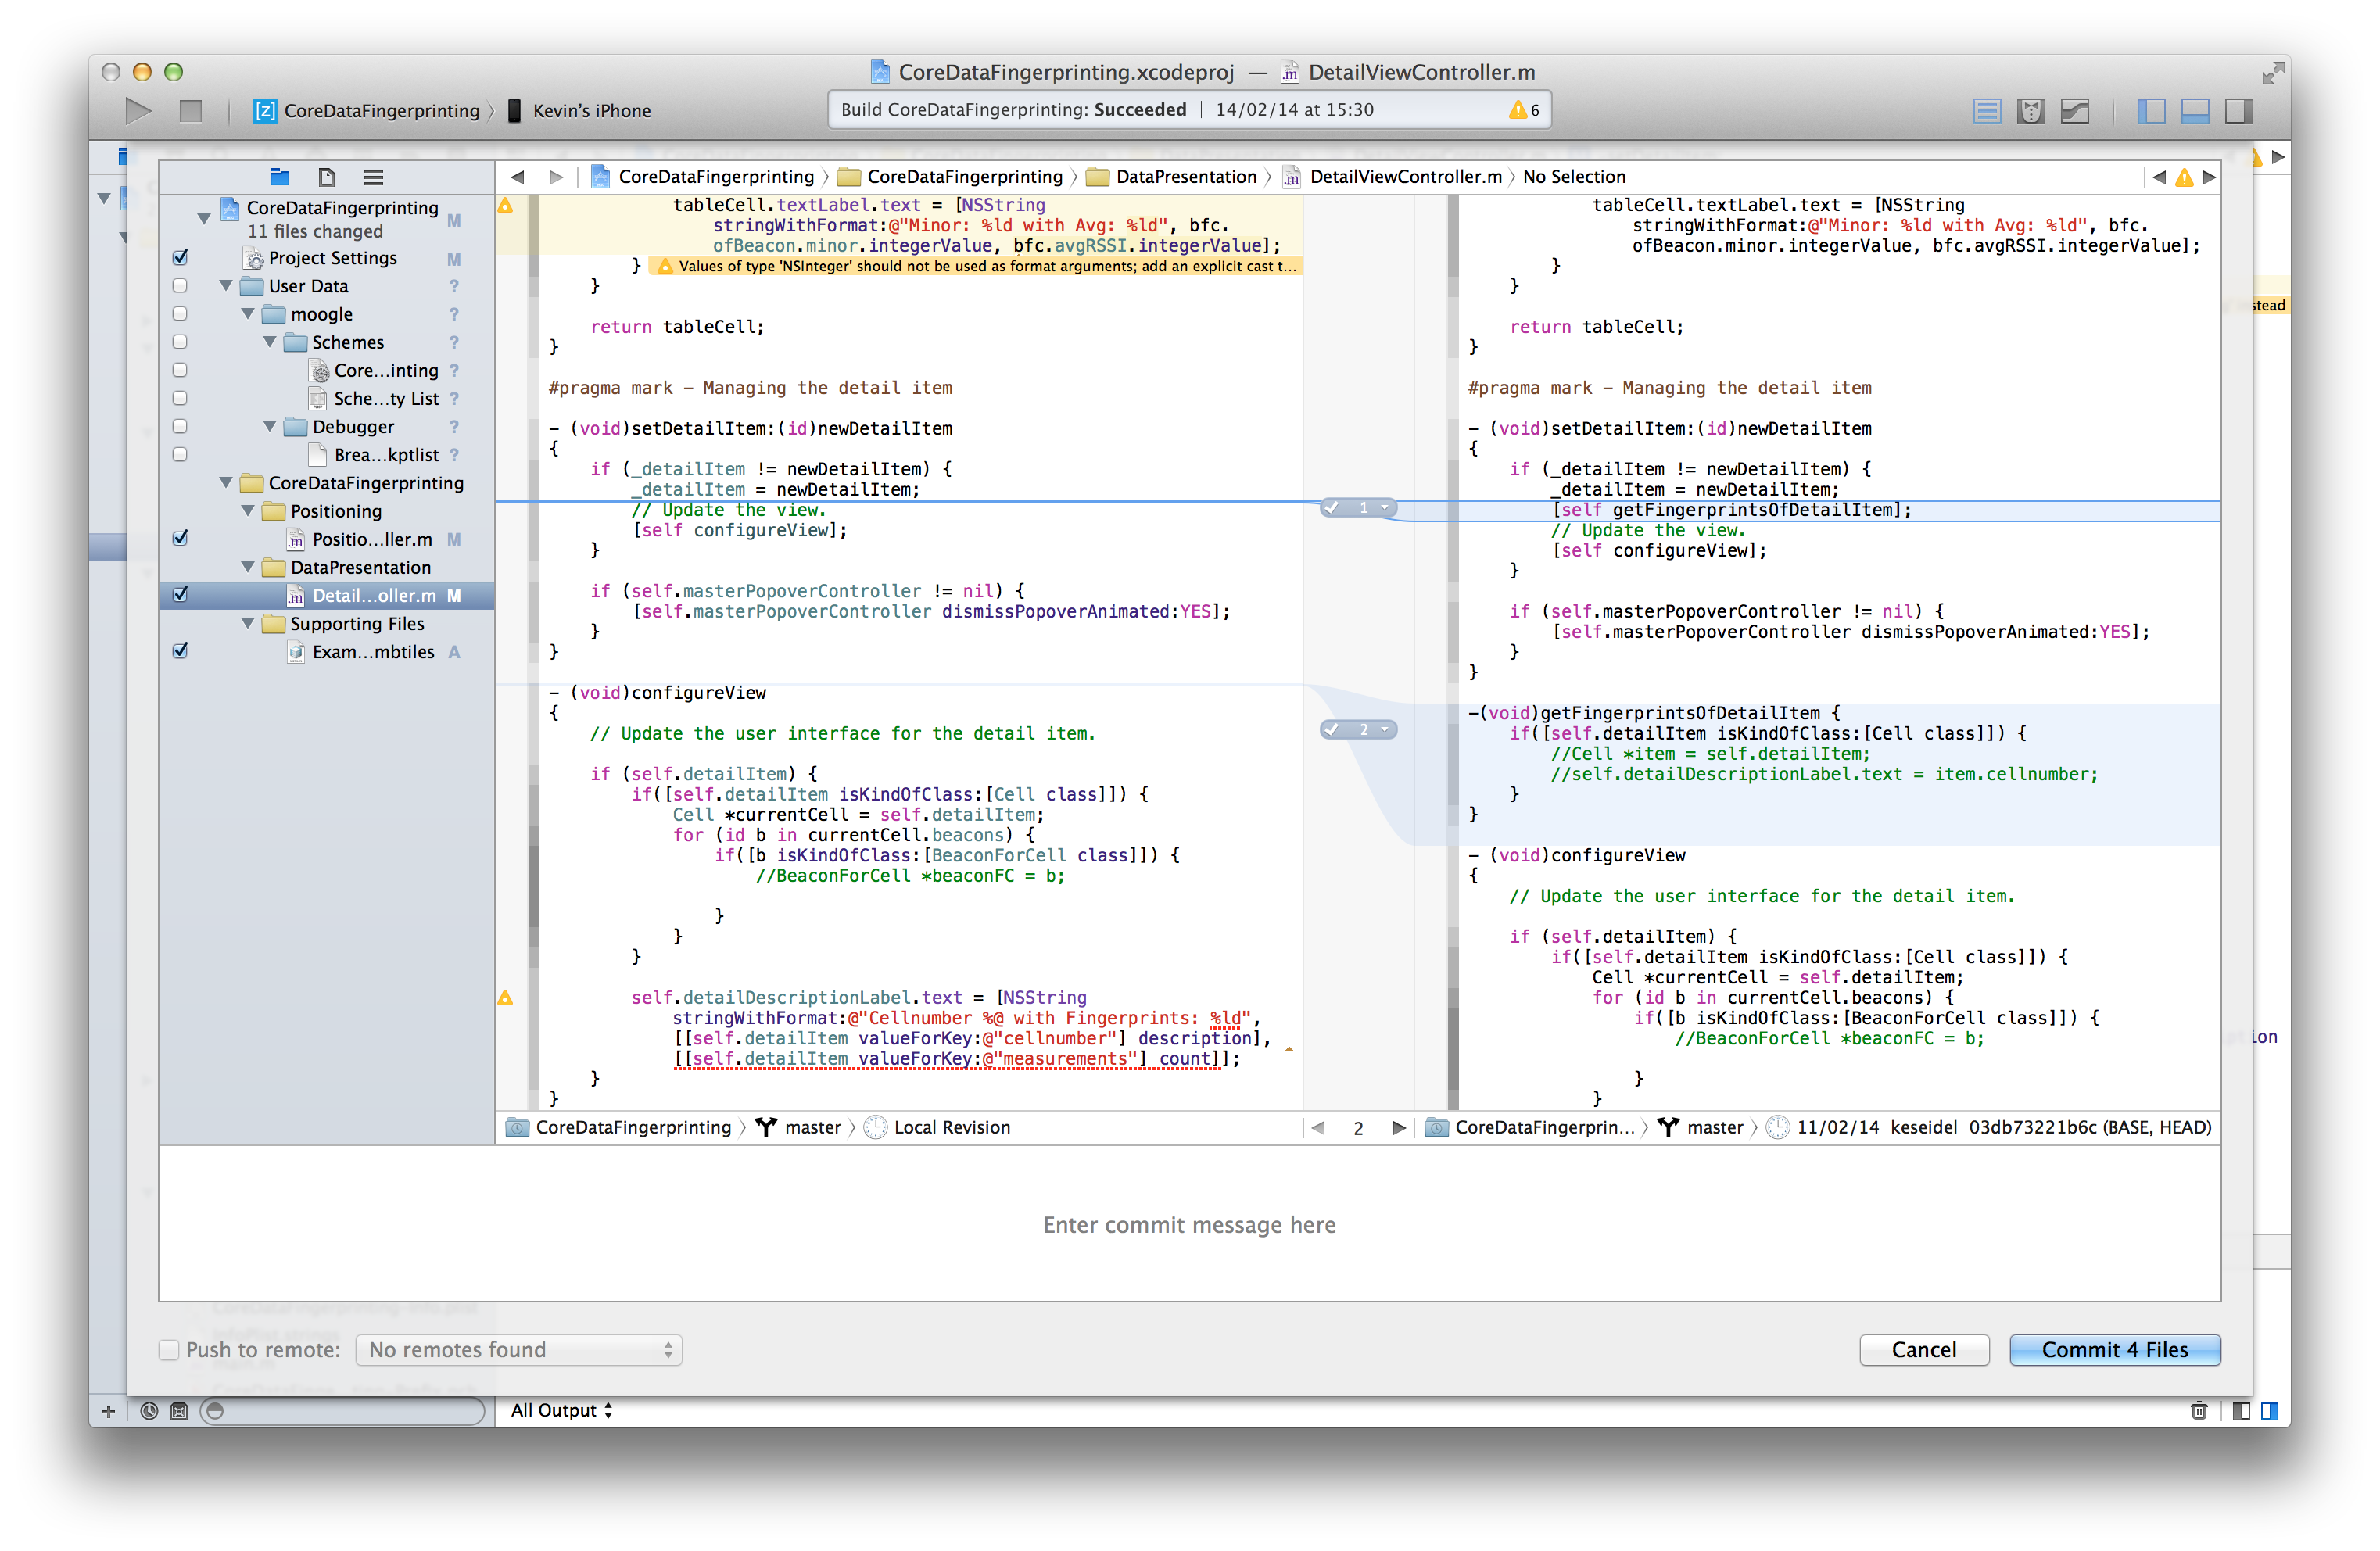
\includegraphics[scale=0.25]{xcode-git-diff}
	\caption{Xcode Versionsverwaltung mit Diff-Anzeige bei einem Commit}
	\label{xcode-git-diff}
\end{figure}


